% Options for packages loaded elsewhere
\PassOptionsToPackage{unicode}{hyperref}
\PassOptionsToPackage{hyphens}{url}
%
\documentclass[
  ignorenonframetext,
]{beamer}
\usepackage{pgfpages}
\setbeamertemplate{caption}[numbered]
\setbeamertemplate{caption label separator}{: }
\setbeamercolor{caption name}{fg=normal text.fg}
\beamertemplatenavigationsymbolsempty
% Prevent slide breaks in the middle of a paragraph
\widowpenalties 1 10000
\raggedbottom
\setbeamertemplate{part page}{
  \centering
  \begin{beamercolorbox}[sep=16pt,center]{part title}
    \usebeamerfont{part title}\insertpart\par
  \end{beamercolorbox}
}
\setbeamertemplate{section page}{
  \centering
  \begin{beamercolorbox}[sep=12pt,center]{part title}
    \usebeamerfont{section title}\insertsection\par
  \end{beamercolorbox}
}
\setbeamertemplate{subsection page}{
  \centering
  \begin{beamercolorbox}[sep=8pt,center]{part title}
    \usebeamerfont{subsection title}\insertsubsection\par
  \end{beamercolorbox}
}
\AtBeginPart{
  \frame{\partpage}
}
\AtBeginSection{
  \ifbibliography
  \else
    \frame{\sectionpage}
  \fi
}
\AtBeginSubsection{
  \frame{\subsectionpage}
}
\usepackage{amsmath,amssymb}
\usepackage{iftex}
\ifPDFTeX
  \usepackage[T1]{fontenc}
  \usepackage[utf8]{inputenc}
  \usepackage{textcomp} % provide euro and other symbols
\else % if luatex or xetex
  \usepackage{unicode-math} % this also loads fontspec
  \defaultfontfeatures{Scale=MatchLowercase}
  \defaultfontfeatures[\rmfamily]{Ligatures=TeX,Scale=1}
\fi
\usepackage{lmodern}
\usetheme[]{Madrid}
\ifPDFTeX\else
  % xetex/luatex font selection
\fi
% Use upquote if available, for straight quotes in verbatim environments
\IfFileExists{upquote.sty}{\usepackage{upquote}}{}
\IfFileExists{microtype.sty}{% use microtype if available
  \usepackage[]{microtype}
  \UseMicrotypeSet[protrusion]{basicmath} % disable protrusion for tt fonts
}{}
\makeatletter
\@ifundefined{KOMAClassName}{% if non-KOMA class
  \IfFileExists{parskip.sty}{%
    \usepackage{parskip}
  }{% else
    \setlength{\parindent}{0pt}
    \setlength{\parskip}{6pt plus 2pt minus 1pt}}
}{% if KOMA class
  \KOMAoptions{parskip=half}}
\makeatother
\usepackage{xcolor}
\newif\ifbibliography
\usepackage{color}
\usepackage{fancyvrb}
\newcommand{\VerbBar}{|}
\newcommand{\VERB}{\Verb[commandchars=\\\{\}]}
\DefineVerbatimEnvironment{Highlighting}{Verbatim}{commandchars=\\\{\}}
% Add ',fontsize=\small' for more characters per line
\usepackage{framed}
\definecolor{shadecolor}{RGB}{248,248,248}
\newenvironment{Shaded}{\begin{snugshade}}{\end{snugshade}}
\newcommand{\AlertTok}[1]{\textcolor[rgb]{0.94,0.16,0.16}{#1}}
\newcommand{\AnnotationTok}[1]{\textcolor[rgb]{0.56,0.35,0.01}{\textbf{\textit{#1}}}}
\newcommand{\AttributeTok}[1]{\textcolor[rgb]{0.13,0.29,0.53}{#1}}
\newcommand{\BaseNTok}[1]{\textcolor[rgb]{0.00,0.00,0.81}{#1}}
\newcommand{\BuiltInTok}[1]{#1}
\newcommand{\CharTok}[1]{\textcolor[rgb]{0.31,0.60,0.02}{#1}}
\newcommand{\CommentTok}[1]{\textcolor[rgb]{0.56,0.35,0.01}{\textit{#1}}}
\newcommand{\CommentVarTok}[1]{\textcolor[rgb]{0.56,0.35,0.01}{\textbf{\textit{#1}}}}
\newcommand{\ConstantTok}[1]{\textcolor[rgb]{0.56,0.35,0.01}{#1}}
\newcommand{\ControlFlowTok}[1]{\textcolor[rgb]{0.13,0.29,0.53}{\textbf{#1}}}
\newcommand{\DataTypeTok}[1]{\textcolor[rgb]{0.13,0.29,0.53}{#1}}
\newcommand{\DecValTok}[1]{\textcolor[rgb]{0.00,0.00,0.81}{#1}}
\newcommand{\DocumentationTok}[1]{\textcolor[rgb]{0.56,0.35,0.01}{\textbf{\textit{#1}}}}
\newcommand{\ErrorTok}[1]{\textcolor[rgb]{0.64,0.00,0.00}{\textbf{#1}}}
\newcommand{\ExtensionTok}[1]{#1}
\newcommand{\FloatTok}[1]{\textcolor[rgb]{0.00,0.00,0.81}{#1}}
\newcommand{\FunctionTok}[1]{\textcolor[rgb]{0.13,0.29,0.53}{\textbf{#1}}}
\newcommand{\ImportTok}[1]{#1}
\newcommand{\InformationTok}[1]{\textcolor[rgb]{0.56,0.35,0.01}{\textbf{\textit{#1}}}}
\newcommand{\KeywordTok}[1]{\textcolor[rgb]{0.13,0.29,0.53}{\textbf{#1}}}
\newcommand{\NormalTok}[1]{#1}
\newcommand{\OperatorTok}[1]{\textcolor[rgb]{0.81,0.36,0.00}{\textbf{#1}}}
\newcommand{\OtherTok}[1]{\textcolor[rgb]{0.56,0.35,0.01}{#1}}
\newcommand{\PreprocessorTok}[1]{\textcolor[rgb]{0.56,0.35,0.01}{\textit{#1}}}
\newcommand{\RegionMarkerTok}[1]{#1}
\newcommand{\SpecialCharTok}[1]{\textcolor[rgb]{0.81,0.36,0.00}{\textbf{#1}}}
\newcommand{\SpecialStringTok}[1]{\textcolor[rgb]{0.31,0.60,0.02}{#1}}
\newcommand{\StringTok}[1]{\textcolor[rgb]{0.31,0.60,0.02}{#1}}
\newcommand{\VariableTok}[1]{\textcolor[rgb]{0.00,0.00,0.00}{#1}}
\newcommand{\VerbatimStringTok}[1]{\textcolor[rgb]{0.31,0.60,0.02}{#1}}
\newcommand{\WarningTok}[1]{\textcolor[rgb]{0.56,0.35,0.01}{\textbf{\textit{#1}}}}
\usepackage{graphicx}
\makeatletter
\def\maxwidth{\ifdim\Gin@nat@width>\linewidth\linewidth\else\Gin@nat@width\fi}
\def\maxheight{\ifdim\Gin@nat@height>\textheight\textheight\else\Gin@nat@height\fi}
\makeatother
% Scale images if necessary, so that they will not overflow the page
% margins by default, and it is still possible to overwrite the defaults
% using explicit options in \includegraphics[width, height, ...]{}
\setkeys{Gin}{width=\maxwidth,height=\maxheight,keepaspectratio}
% Set default figure placement to htbp
\makeatletter
\def\fps@figure{htbp}
\makeatother
\setlength{\emergencystretch}{3em} % prevent overfull lines
\providecommand{\tightlist}{%
  \setlength{\itemsep}{0pt}\setlength{\parskip}{0pt}}
\setcounter{secnumdepth}{-\maxdimen} % remove section numbering
\logo{
\includegraphics[height=1cm,width=3cm]{logo.png}}
\usetheme{Madrid}
\usefonttheme{serif}
\setbeamertemplate{navigation symbols}{}

\usepackage{amsmath}

\usepackage{graphicx}
\setkeys{Gin}{width=0.5\linewidth} 


\usepackage{booktabs}
\usepackage{longtable}
\usepackage{array}
\usepackage{multirow}
\usepackage{wrapfig}
\usepackage{float}
\usepackage{colortbl}
\usepackage{pdflscape}
\usepackage{tabu}
\usepackage{threeparttable}
\usepackage{threeparttablex}
\usepackage[normalem]{ulem}
\usepackage{makecell}
\usepackage{xcolor}
\ifLuaTeX
  \usepackage{selnolig}  % disable illegal ligatures
\fi
\usepackage{bookmark}
\IfFileExists{xurl.sty}{\usepackage{xurl}}{} % add URL line breaks if available
\urlstyle{same}
\hypersetup{
  pdftitle={Lecture 2},
  pdfauthor={Endri Raco},
  hidelinks,
  pdfcreator={LaTeX via pandoc}}

\title{Lecture 2}
\subtitle{Data Visualization with ggplot2}
\author{Endri Raco}
\date{10 February, 2025}

\begin{document}
\frame{\titlepage}

\begin{frame}[allowframebreaks]
  \tableofcontents[hideallsubsections]
\end{frame}
\section{Introduction}\label{introduction}

\begin{frame}{The grammar of graphics}
\phantomsection\label{the-grammar-of-graphics}
The first step in thinking creatively about data visualization is to
appreciate that graphics are built upon an underlying grammar.
\end{frame}

\begin{frame}[fragile]{The quick brown fox jumps over the lazy dog}
\phantomsection\label{the-quick-brown-fox-jumps-over-the-lazy-dog}
\begin{verbatim}
- To begin, let's consider one of the most well-known sentences in English. 

- The quick brown fox jumps over the lazy dog.
\end{verbatim}
\end{frame}

\begin{frame}[fragile]{The quick brown fox jumps over the lazy dog}
\phantomsection\label{the-quick-brown-fox-jumps-over-the-lazy-dog-1}
\begin{verbatim}
- Every word in the sentence has a clear grammatical definition and when we write text, we take great care to choose the grammatical elements so that we communicate a very specific message. 
\end{verbatim}

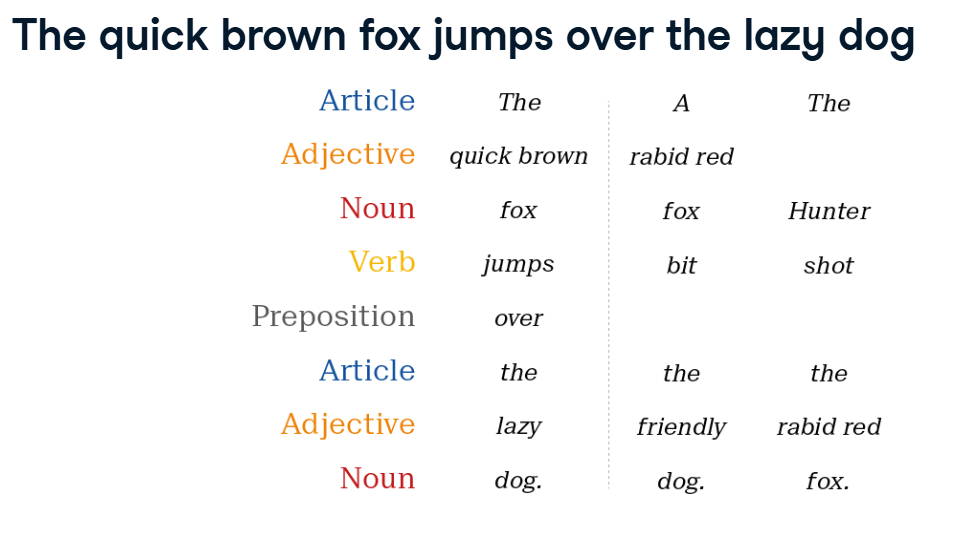
\includegraphics{../images/im120.png}
\end{frame}

\begin{frame}[fragile]{Grammar of graphics}
\phantomsection\label{grammar-of-graphics}
\begin{verbatim}
- If we changed any of the grammatical elements of this sentence it would change the meaning, sometimes subtly, sometimes dramatically.

- The same concept holds true for data visualization - graphics are built on an underlying grammar. 
\end{verbatim}
\end{frame}

\begin{frame}[fragile]{Grammar of graphics}
\phantomsection\label{grammar-of-graphics-1}
\begin{verbatim}
- The grammar of graphics is a plotting framework developed by Leland Wilkinson and published in his 1999 book, *The Grammar of Graphics*. 
\end{verbatim}

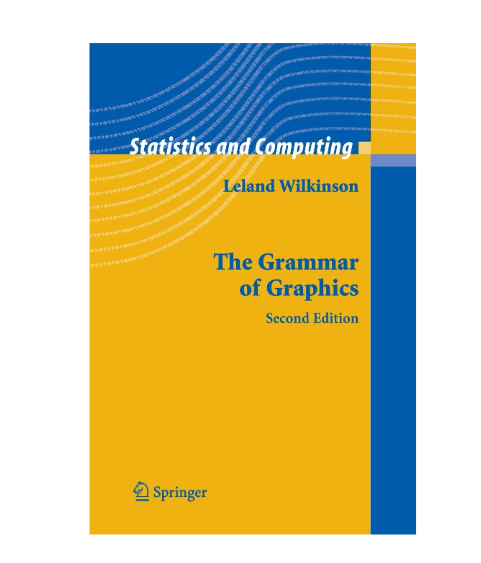
\includegraphics{../images/im121.png}
\end{frame}

\begin{frame}[fragile]{Grammar of graphics}
\phantomsection\label{grammar-of-graphics-2}
There are two key things to note about the grammar of graphics.

\begin{verbatim}
- First, graphics are made up of distinct layers of grammatical elements, 

- Second, meaningful plots are built around appropriate aesthetic mappings. 
\end{verbatim}
\end{frame}

\begin{frame}{Grammar of graphics}
\phantomsection\label{grammar-of-graphics-3}
\begin{itemize}
\tightlist
\item
  To continue our analogy to written grammar, the layers are like the
  adjectives and nouns and the aesthetic mappings are like the
  grammatical rules for how to assemble that vocabulary.
\end{itemize}
\end{frame}

\begin{frame}{The three essential grammatical elements}
\phantomsection\label{the-three-essential-grammatical-elements}
Let's explore grammatical elements first.
\end{frame}

\begin{frame}{The three essential grammatical elements}
\phantomsection\label{the-three-essential-grammatical-elements-1}
There are three essential grammatical elements: data, aesthetics, and
geometries.

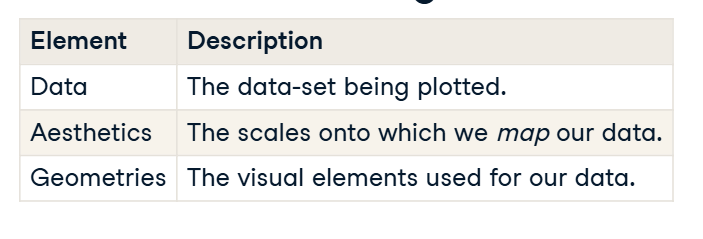
\includegraphics{../images/im122.png}
\end{frame}

\begin{frame}{The three essential grammatical elements}
\phantomsection\label{the-three-essential-grammatical-elements-2}
\begin{itemize}
\item
  The data is obviously the data which we want to plot.

  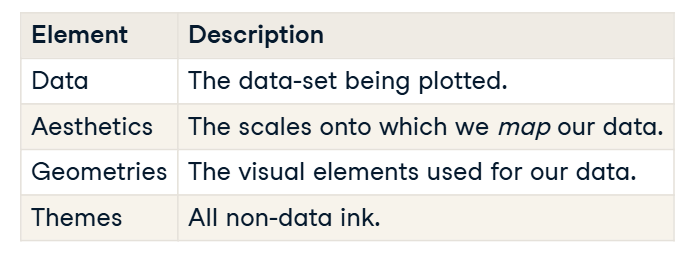
\includegraphics{../images/im123.png}
\end{itemize}

\#\# The three essential grammatical elements

\begin{itemize}
\tightlist
\item
  The aesthetics layer refers to the scales onto which we will map our
  data, and the geom layer refers to the actual shape the data will take
  in the plot.
\end{itemize}

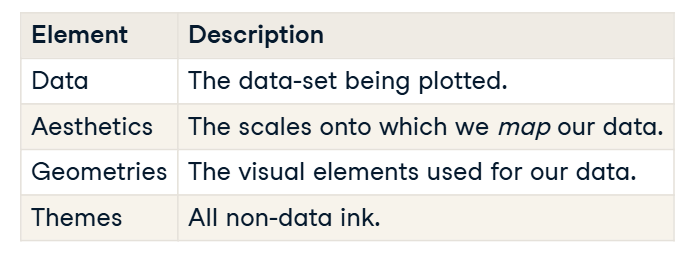
\includegraphics{../images/im123.png}

\#\# The three essential grammatical elements

\begin{itemize}
\tightlist
\item
  The geom layer refers to the actual shape the data will take in the
  plot.
\end{itemize}

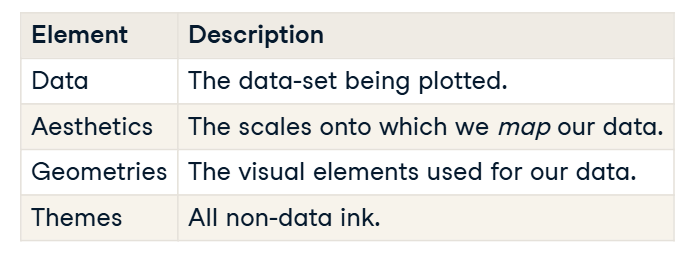
\includegraphics{../images/im123.png}
\end{frame}

\begin{frame}{Core competency}
\phantomsection\label{core-competency}
The rest are optional layers.

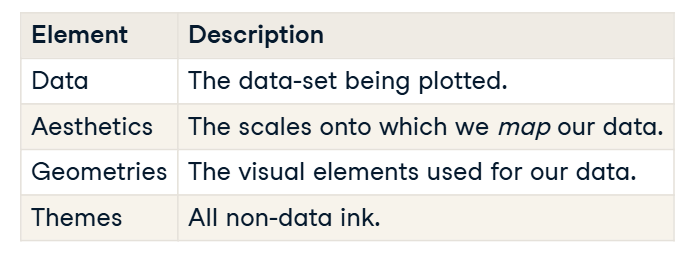
\includegraphics{../images/im123.png}

This includes the theme layer, which controls all the non-data ink. In
this lecture, we'll cover these first four layers which will comprise
your core competency.
\end{frame}

\begin{frame}{The seven grammatical elements}
\phantomsection\label{the-seven-grammatical-elements}
In the next lecture we'll explore the remaining grammatical elements:
the statistics, coordinates and facets layers.

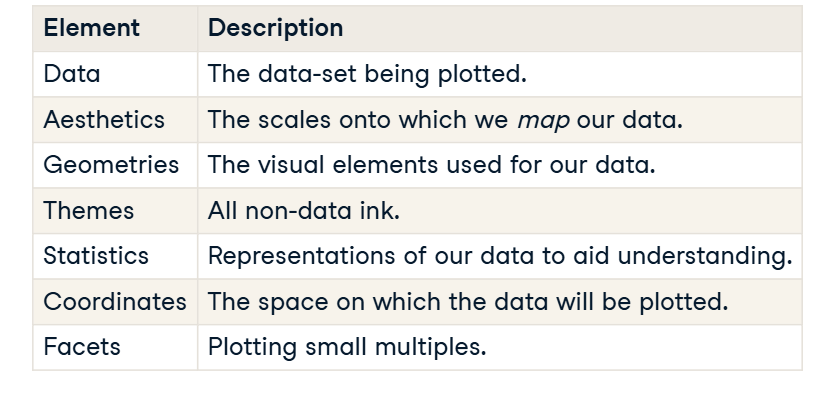
\includegraphics{../images/im124.png}
\end{frame}

\begin{frame}{Jargon for each element}
\phantomsection\label{jargon-for-each-element}
This diagram gives an example of some of the terms we'll encounter in
each element.

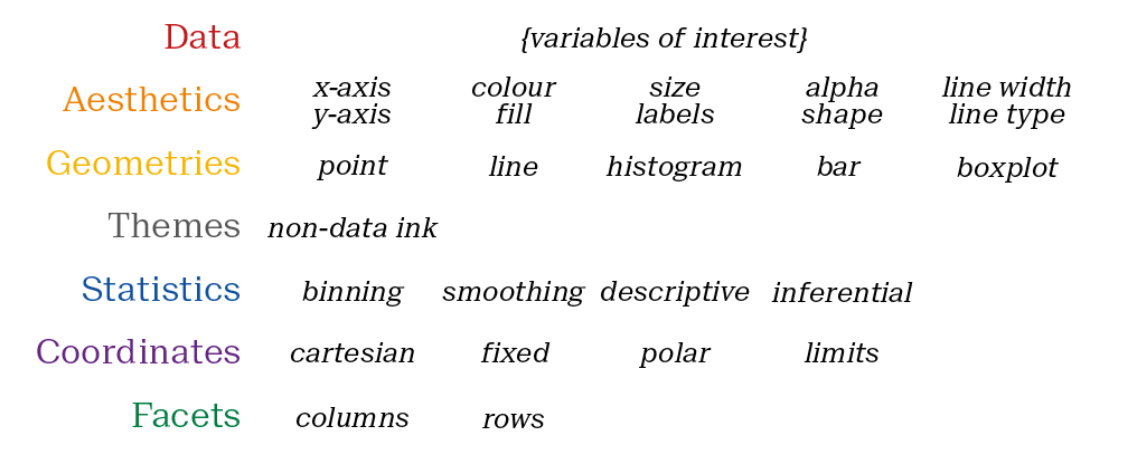
\includegraphics{../images/im125.png}
\end{frame}

\begin{frame}[fragile]{Jargon for each element}
\phantomsection\label{jargon-for-each-element-1}
\begin{verbatim}
- Whenever we make a plot we are choosing among these options and many others not displayed. 

- By the end of this lecture you'll be able to generate meaningful and publication-quality exploratory plots using       the first four layers.
\end{verbatim}
\end{frame}

\begin{frame}{ggplot2 layers}
\phantomsection\label{ggplot2-layers}
Now that we have some idea about the different grammatical elements of
graphics, let's see how this works in practice.
\end{frame}

\begin{frame}{ggplot2 package}
\phantomsection\label{ggplot2-package}
\begin{itemize}
\item
  The grammar of graphic is implemented in R using the ggplot2 package.
\item
  There are two key functions that ggplot2 serves.
\end{itemize}
\end{frame}

\begin{frame}{ggplot2 package}
\phantomsection\label{ggplot2-package-1}
\begin{itemize}
\item
  First, we construct plots by layering grammatical elements on top of
  each other.
\item
  Second, we use aesthetic mappings to bridge the link between data and
  it's visual interpretation.
\end{itemize}
\end{frame}

\begin{frame}{ggplot2 package}
\phantomsection\label{ggplot2-package-2}
\begin{itemize}
\item
  We are going to go through each grammatical element in depth in this
  and the next lecture.
\item
  Here I'll introduce a data set which will be used throughout the
  videos and we'll go over some simple examples.
\end{itemize}
\end{frame}

\begin{frame}{Data}
\phantomsection\label{data}
The bottom layer is the data element.

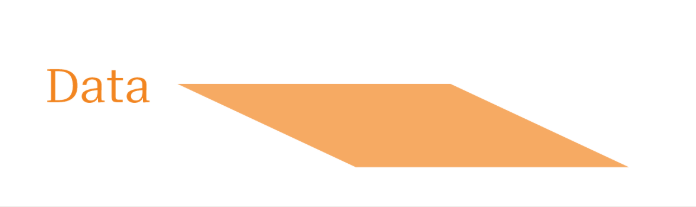
\includegraphics{../images/im126.png}
\end{frame}

\begin{frame}{Data}
\phantomsection\label{data-1}
\begin{itemize}
\item
  Obviously we need some data to plot.
\item
  I'm going to use several different data sets in the course videos,
\end{itemize}
\end{frame}

\begin{frame}{Iris dataset}
\phantomsection\label{iris-dataset}
One of which is the classic iris data set collected by Edgar Anderson in
the 1930s and thereafter popularized by Ronald Fisher.

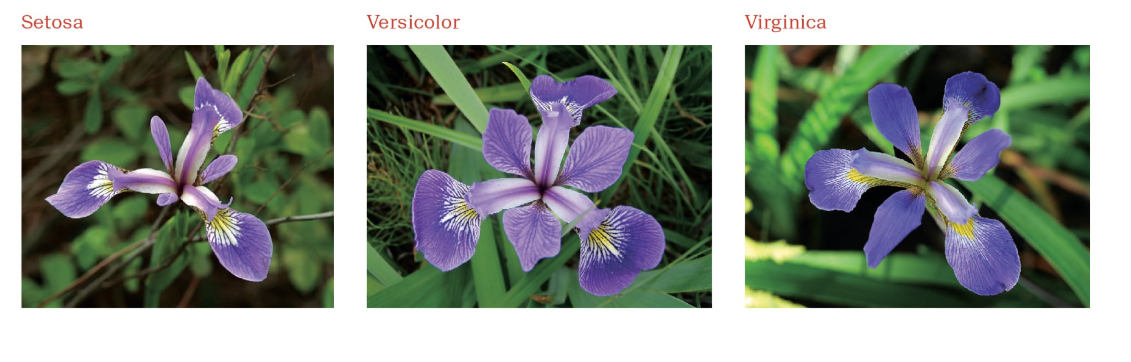
\includegraphics{../images/im127.png}
\end{frame}

\begin{frame}{Iris dataset}
\phantomsection\label{iris-dataset-1}
\begin{itemize}
\item
  The data set contains information on three iris species, setosa,
  versicolor, and virginica.
\item
  Four measurements were taken from each plant - the petal length and
  width and the sepal length and width.
\end{itemize}
\end{frame}

\begin{frame}{Iris dataset}
\phantomsection\label{iris-dataset-2}
\begin{itemize}
\item
  You're probably familiar with petals, they're the colorful part of a
  flower.
\item
  Sepals are the outer leaves of the flower, they are typically green,
  but in this case they're also colorful.
\item
  There are 50 specimens of each species.
\end{itemize}
\end{frame}

\begin{frame}{Iris dataset}
\phantomsection\label{iris-dataset-3}
The data is stored in an object called \textbf{iris}, there are five
variables: the species and one for each of the properties which were
measured.

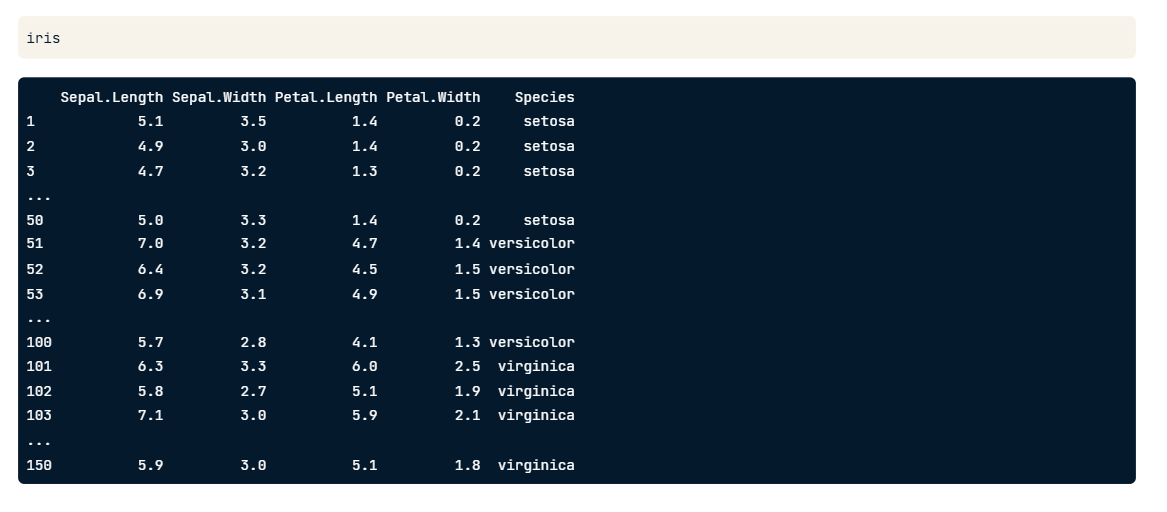
\includegraphics{../images/im128.png}
\end{frame}

\begin{frame}{Aesthetics}
\phantomsection\label{aesthetics}
The next layer we'll add is the aesthetics element, which tells us which
scales we should map our data onto.


\includegraphics{../images/im129.png}
\end{frame}

\begin{frame}{Aesthetics}
\phantomsection\label{aesthetics-1}
\begin{itemize}
\item
  This is where the second main component of the grammar of graphics
  comes into play.
\item
  On top of layering the grammatical elements, it's here that we
  establish our aesthetic mappings.
\end{itemize}
\end{frame}

\begin{frame}{Iris aesthetics}
\phantomsection\label{iris-aesthetics}
In this case we are going to make a scatter plot so we're going to map
Sepal-dot-Length onto the X aesthetic and Sepal-dot-Width onto the Y
aesthetic.

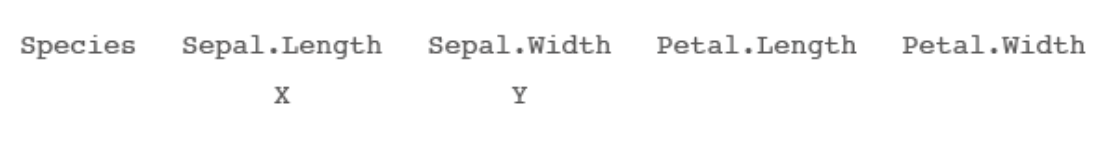
\includegraphics{../images/im130.png}
\end{frame}

\begin{frame}{Geometries}
\phantomsection\label{geometries}
The next element is the geometry element.

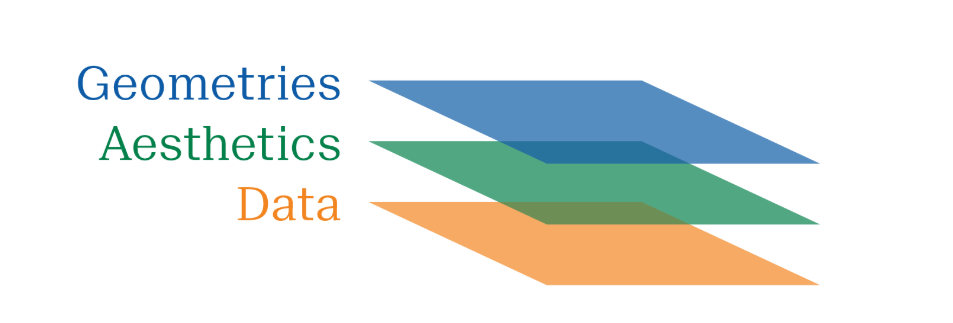
\includegraphics{../images/im131.png}

This allows us to choose how the plot will look.
\end{frame}

\begin{frame}{Iris geometries}
\phantomsection\label{iris-geometries}
After we've established our three essential layers, we have enough
instructions to make a basic scatter plot.

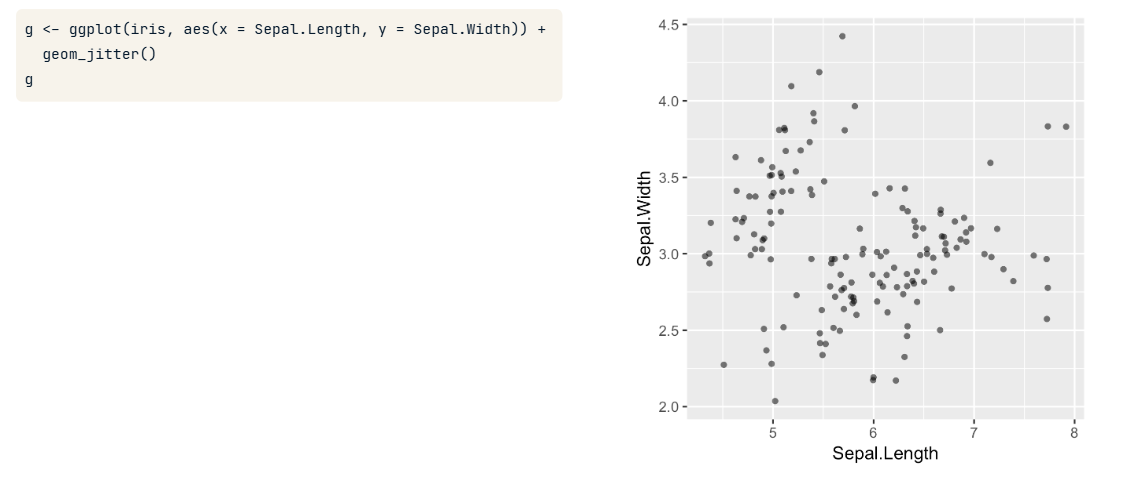
\includegraphics{../images/im132.png}

It's pretty rough, so to get a more meaningful and cleaner
visualization, we'll have to use the other layers.
\end{frame}

\begin{frame}{Themes}
\phantomsection\label{themes}
The next layer we'll look at is the themes element.

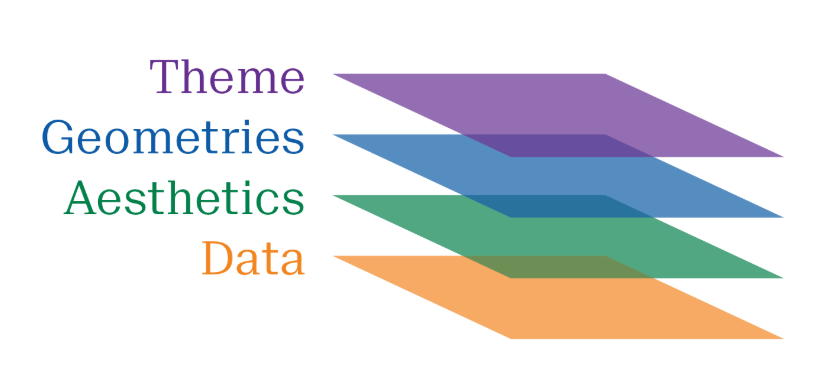
\includegraphics{../images/im133.png}
\end{frame}

\begin{frame}{Themes}
\phantomsection\label{themes-1}
It controls all the non-data ink on our plot.
\end{frame}

\begin{frame}{Iris themes}
\phantomsection\label{iris-themes}
Which allows us to get a nice looking, meaningful and
publication-quality plot directly in R.

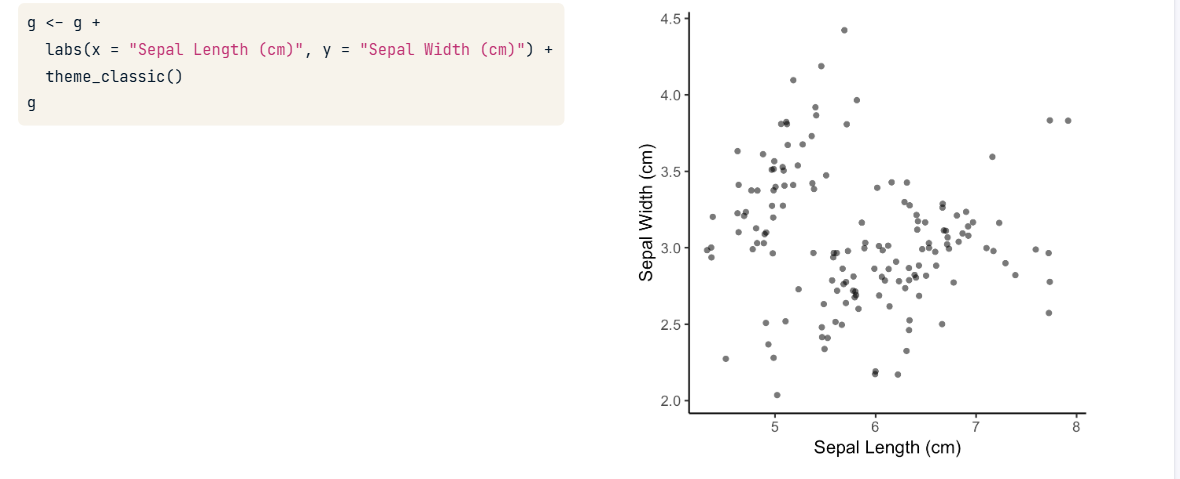
\includegraphics{../images/im134.png}
\end{frame}

\begin{frame}{Practice: Introduction to Geometries in ggplot2}
\phantomsection\label{practice-introduction-to-geometries-in-ggplot2}
\begin{itemize}
\tightlist
\item
  In this exercise, we'll work with the \textbf{diamonds} dataset.
\item
  The goal is to explore and plot the data using ggplot2.
\end{itemize}
\end{frame}

\begin{frame}[fragile]{Practice: The diamonds dataset}
\phantomsection\label{practice-the-diamonds-dataset}
\begin{itemize}
\tightlist
\item
  The \textbf{diamonds} dataset contains information on 1,000 diamonds.
\item
  Some key variables include:

  \begin{itemize}
  \tightlist
  \item
    \texttt{carat}: A measurement of the diamond's size.
  \item
    \texttt{price}: The price of the diamond in dollars.
  \end{itemize}
\end{itemize}
\end{frame}

\begin{frame}[fragile]{Step 1: Explore the dataset}
\phantomsection\label{step-1-explore-the-dataset}
Use the \texttt{str()} function to inspect the structure of the
\textbf{diamonds} dataset.

\AddToHookNext{env/Highlighting/begin}{\tiny}

\begin{Shaded}
\begin{Highlighting}[]
\CommentTok{\# Load ggplot2 package}
\FunctionTok{library}\NormalTok{(ggplot2)}

\CommentTok{\# Explore the structure of the diamonds dataset}
\FunctionTok{str}\NormalTok{(diamonds)}
\end{Highlighting}
\end{Shaded}

\begin{verbatim}
tibble [53,940 x 10] (S3: tbl_df/tbl/data.frame)
 $ carat  : num [1:53940] 0.23 0.21 0.23 0.29 0.31 0.24 0.24 0.26 0.22 0.23 ...
 $ cut    : Ord.factor w/ 5 levels "Fair"<"Good"<..: 5 4 2 4 2 3 3 3 1 3 ...
 $ color  : Ord.factor w/ 7 levels "D"<"E"<"F"<"G"<..: 2 2 2 6 7 7 6 5 2 5 ...
 $ clarity: Ord.factor w/ 8 levels "I1"<"SI2"<"SI1"<..: 2 3 5 4 2 6 7 3 4 5 ...
 $ depth  : num [1:53940] 61.5 59.8 56.9 62.4 63.3 62.8 62.3 61.9 65.1 59.4 ...
 $ table  : num [1:53940] 55 61 65 58 58 57 57 55 61 61 ...
 $ price  : int [1:53940] 326 326 327 334 335 336 336 337 337 338 ...
 $ x      : num [1:53940] 3.95 3.89 4.05 4.2 4.34 3.94 3.95 4.07 3.87 4 ...
 $ y      : num [1:53940] 3.98 3.84 4.07 4.23 4.35 3.96 3.98 4.11 3.78 4.05 ...
 $ z      : num [1:53940] 2.43 2.31 2.31 2.63 2.75 2.48 2.47 2.53 2.49 2.39 ...
\end{verbatim}
\end{frame}

\begin{frame}[fragile]{Step 2: Create a basic plot}
\phantomsection\label{step-2-create-a-basic-plot}
Use ggplot() to create a basic plot of carat (x-axis) vs.~price
(y-axis).

\AddToHookNext{env/Highlighting/begin}{\tiny}

\begin{Shaded}
\begin{Highlighting}[]
\CommentTok{\# Basic ggplot setup}
\FunctionTok{ggplot}\NormalTok{(}\AttributeTok{data =}\NormalTok{ diamonds, }\FunctionTok{aes}\NormalTok{(}\AttributeTok{x =}\NormalTok{ carat, }\AttributeTok{y =}\NormalTok{ price))}
\end{Highlighting}
\end{Shaded}

\begin{center}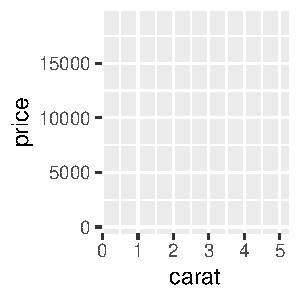
\includegraphics[width=0.5\linewidth]{Figs/unnamed-chunk-2-1} \end{center}
\end{frame}

\begin{frame}[fragile]{Step 3: Add points to the plot}
\phantomsection\label{step-3-add-points-to-the-plot}
Use the geom\_point() function to add a scatter plot layer.

\AddToHookNext{env/Highlighting/begin}{\tiny}

\begin{Shaded}
\begin{Highlighting}[]
\CommentTok{\# Add points to the plot}
\FunctionTok{ggplot}\NormalTok{(}\AttributeTok{data =}\NormalTok{ diamonds, }\FunctionTok{aes}\NormalTok{(}\AttributeTok{x =}\NormalTok{ carat, }\AttributeTok{y =}\NormalTok{ price)) }\SpecialCharTok{+} \FunctionTok{geom\_point}\NormalTok{()}
\end{Highlighting}
\end{Shaded}

\begin{center}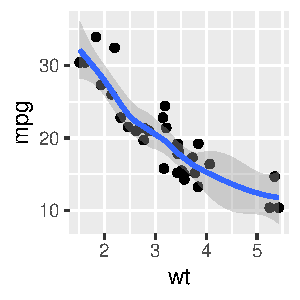
\includegraphics[width=0.5\linewidth]{Figs/unnamed-chunk-3-1} \end{center}
\end{frame}

\begin{frame}[fragile]{Step 4: Add a smooth trend line}
\phantomsection\label{step-4-add-a-smooth-trend-line}
Use the geom\_smooth() function to add a smooth trend curve to the plot.

\AddToHookNext{env/Highlighting/begin}{\tiny}

\begin{Shaded}
\begin{Highlighting}[]
\CommentTok{\# Add points and a smooth trend line}
\FunctionTok{ggplot}\NormalTok{(}\AttributeTok{data =}\NormalTok{ diamonds, }\FunctionTok{aes}\NormalTok{(}\AttributeTok{x =}\NormalTok{ carat, }\AttributeTok{y =}\NormalTok{ price)) }\SpecialCharTok{+} \FunctionTok{geom\_point}\NormalTok{() }\SpecialCharTok{+}
    \FunctionTok{geom\_smooth}\NormalTok{()}
\end{Highlighting}
\end{Shaded}

\begin{center}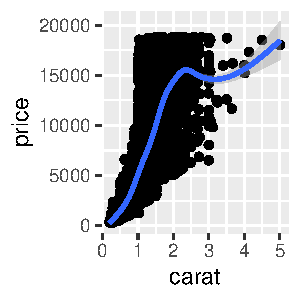
\includegraphics[width=0.5\linewidth]{Figs/unnamed-chunk-4-1} \end{center}
\end{frame}

\begin{frame}[fragile]{Customizing ggplot2 Geometries}
\phantomsection\label{customizing-ggplot2-geometries}
\begin{itemize}
\tightlist
\item
  Learn how to customize \textbf{ggplot2} geometries.
\item
  Modify aesthetics such as \texttt{color} and \texttt{alpha}.
\end{itemize}
\end{frame}

\begin{frame}[fragile]{Practice 2: Map \texttt{color} to
\texttt{clarity}}
\phantomsection\label{practice-2-map-color-to-clarity}
\begin{itemize}
\tightlist
\item
  \textbf{Objective}: Map the \texttt{color} aesthetic to the
  \texttt{clarity} variable.
\item
  This will create a color-coded scatter plot based on diamond clarity.
\end{itemize}
\end{frame}

\begin{frame}[fragile]{Practice 2: Map \texttt{color} to
\texttt{clarity}}
\phantomsection\label{practice-2-map-color-to-clarity-1}
\AddToHookNext{env/Highlighting/begin}{\tiny}

\begin{Shaded}
\begin{Highlighting}[]
\CommentTok{\# Create a plot with color mapped to clarity}
\FunctionTok{ggplot}\NormalTok{(}\AttributeTok{data =}\NormalTok{ diamonds, }\FunctionTok{aes}\NormalTok{(}\AttributeTok{x =}\NormalTok{ carat, }\AttributeTok{y =}\NormalTok{ price, }\AttributeTok{color =}\NormalTok{ clarity)) }\SpecialCharTok{+}
    \FunctionTok{geom\_point}\NormalTok{() }\SpecialCharTok{+} \FunctionTok{geom\_smooth}\NormalTok{()}
\end{Highlighting}
\end{Shaded}

\begin{center}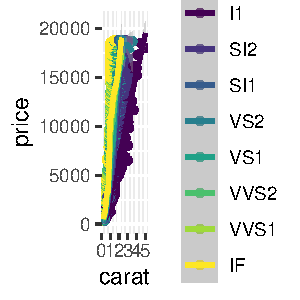
\includegraphics[width=0.5\linewidth]{Figs/unnamed-chunk-5-1} \end{center}
\end{frame}

\begin{frame}{Practice 2: Adjust Transparency with alpha}
\phantomsection\label{practice-2-adjust-transparency-with-alpha}
\begin{itemize}
\tightlist
\item
  \textbf{Objective}: Make points partially transparent.
\item
  Use the alpha argument in geom\_point() to set transparency.
\end{itemize}
\end{frame}

\begin{frame}[fragile]{Practice 2: Adjust Transparency with alpha}
\phantomsection\label{practice-2-adjust-transparency-with-alpha-1}
\AddToHookNext{env/Highlighting/begin}{\tiny}

\begin{Shaded}
\begin{Highlighting}[]
\CommentTok{\# Add transparency to points}
\FunctionTok{ggplot}\NormalTok{(}\AttributeTok{data =}\NormalTok{ diamonds, }\FunctionTok{aes}\NormalTok{(}\AttributeTok{x =}\NormalTok{ carat, }\AttributeTok{y =}\NormalTok{ price, }\AttributeTok{color =}\NormalTok{ clarity)) }\SpecialCharTok{+}
    \FunctionTok{geom\_point}\NormalTok{(}\AttributeTok{alpha =} \FloatTok{0.4}\NormalTok{) }\SpecialCharTok{+} \FunctionTok{geom\_smooth}\NormalTok{()}
\end{Highlighting}
\end{Shaded}

\begin{center}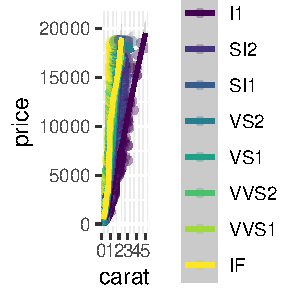
\includegraphics[width=0.5\linewidth]{Figs/unnamed-chunk-6-1} \end{center}
\end{frame}

\begin{frame}{Practice 3: Saving Plots as Variables in ggplot2}
\phantomsection\label{practice-3-saving-plots-as-variables-in-ggplot2}
\begin{itemize}
\tightlist
\item
  In ggplot2, plots can be saved as variables.
\item
  This allows reusing a base plot and adding layers incrementally.
\end{itemize}
\end{frame}

\begin{frame}[fragile]{Practice 3: Create and Save a Basic Plot}
\phantomsection\label{practice-3-create-and-save-a-basic-plot}
\begin{itemize}
\tightlist
\item
  Plot \texttt{price} (y-axis) vs.~\texttt{carat} (x-axis) using the
  diamonds dataset.
\item
  Save the plot to a variable named \texttt{plt\_price\_vs\_carat}.
\end{itemize}
\end{frame}

\begin{frame}[fragile]{Practice 3: Create and Save a Basic Plot}
\phantomsection\label{practice-3-create-and-save-a-basic-plot-1}
\AddToHookNext{env/Highlighting/begin}{\tiny}

\begin{Shaded}
\begin{Highlighting}[]
\CommentTok{\# Load ggplot2}
\FunctionTok{library}\NormalTok{(ggplot2)}

\CommentTok{\# Save a basic ggplot as a variable}
\NormalTok{plt\_price\_vs\_carat }\OtherTok{\textless{}{-}} \FunctionTok{ggplot}\NormalTok{(}\AttributeTok{data =}\NormalTok{ diamonds, }\FunctionTok{aes}\NormalTok{(}\AttributeTok{x =}\NormalTok{ carat,}
    \AttributeTok{y =}\NormalTok{ price))}
\end{Highlighting}
\end{Shaded}
\end{frame}

\begin{frame}[fragile]{Practice 3: Add Layers to the Saved Plot}
\phantomsection\label{practice-3-add-layers-to-the-saved-plot}
Add a point layer to the plot using geom\_point().

\AddToHookNext{env/Highlighting/begin}{\tiny}

\begin{Shaded}
\begin{Highlighting}[]
\CommentTok{\# Add points to the saved plot}
\NormalTok{plt\_price\_vs\_carat }\OtherTok{\textless{}{-}}\NormalTok{ plt\_price\_vs\_carat }\SpecialCharTok{+} \FunctionTok{geom\_point}\NormalTok{()}
\end{Highlighting}
\end{Shaded}
\end{frame}

\begin{frame}[fragile]{Practice 3: Add Layers to the Saved Plot}
\phantomsection\label{practice-3-add-layers-to-the-saved-plot-1}
Display the updated plot stored in plt\_price\_vs\_carat.

\AddToHookNext{env/Highlighting/begin}{\tiny}

\begin{Shaded}
\begin{Highlighting}[]
\CommentTok{\# Display the updated plot}
\NormalTok{plt\_price\_vs\_carat}
\end{Highlighting}
\end{Shaded}

\begin{center}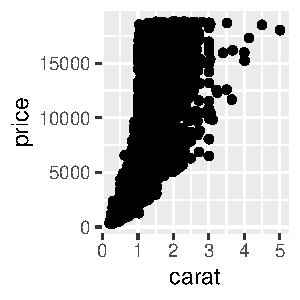
\includegraphics[width=0.5\linewidth]{Figs/unnamed-chunk-9-1} \end{center}
\end{frame}

\begin{frame}{Visible aesthetics}
\phantomsection\label{visible-aesthetics}
In this section we'll explore aesthetics, and understand how they are
distinct from attributes.
\end{frame}

\begin{frame}{Mapping onto the X and Y axes}
\phantomsection\label{mapping-onto-the-x-and-y-axes}
\begin{itemize}
\item
  In ggplot2, the mapping of aesthetics elements is a key concept to
  master.
\item
  So what do we mean by mapping?
\end{itemize}
\end{frame}

\begin{frame}{Mapping onto the X and Y axes}
\phantomsection\label{mapping-onto-the-x-and-y-axes-1}
This becomes clear when we understand that our beloved X and Y axes on a
straightforward scatter plot are aesthetics.

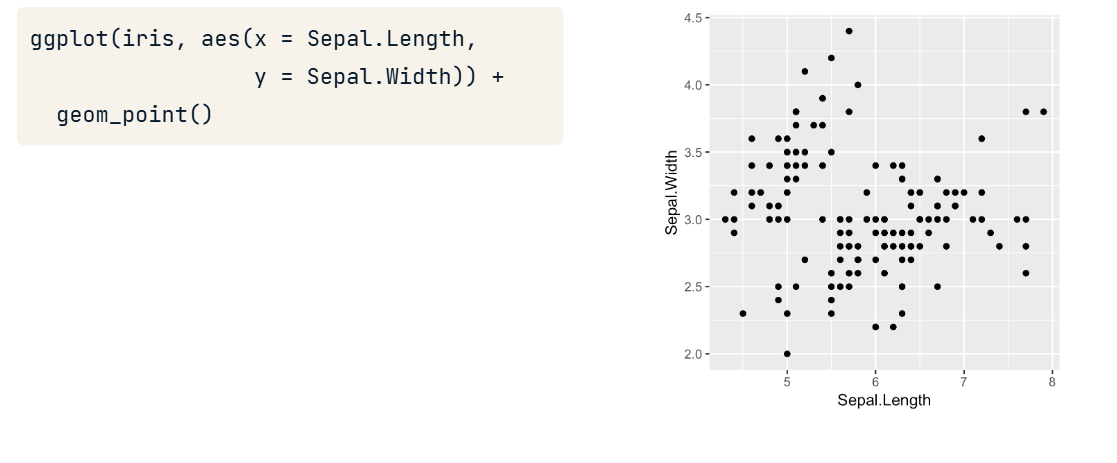
\includegraphics{../images/im135.png}
\end{frame}

\begin{frame}{Mapping onto the X and Y axes}
\phantomsection\label{mapping-onto-the-x-and-y-axes-2}
\begin{itemize}
\item
  They define the position of dots on a common scale, like this example
  we saw in the previous part.
\item
  The sepal length is mapped onto the X axis and the sepal width is
  mapped onto the Y axis.
\end{itemize}
\end{frame}

\begin{frame}{Mapping onto the X and Y axes}
\phantomsection\label{mapping-onto-the-x-and-y-axes-3}
Here, we'll focus on the most common visual aesthetics and but we'll
encounter more throughout the courses.

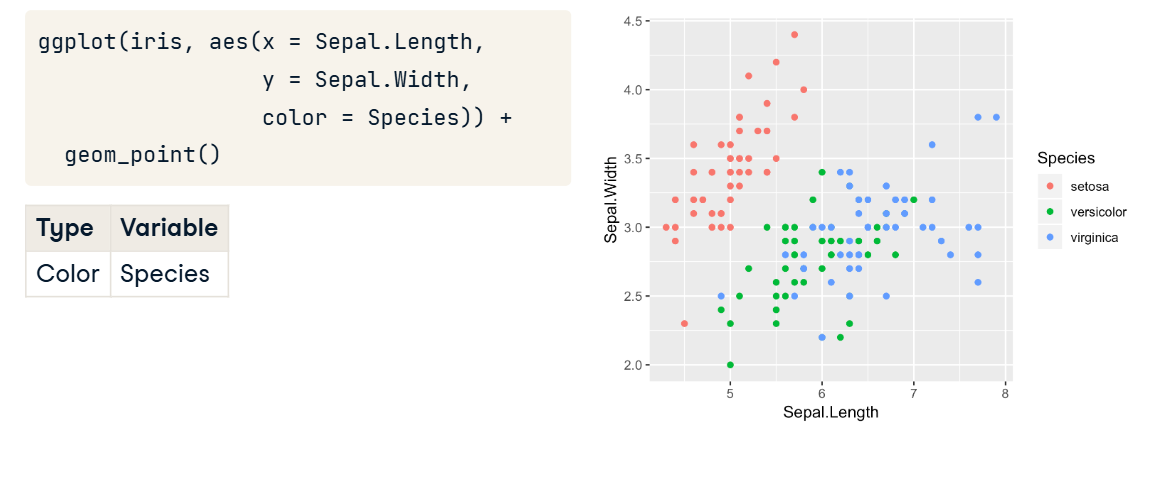
\includegraphics{../images/im136.png}

When making multivariate plots we'll use aesthetics appropriately to
maximize the number of variables we can add to a plot.
\end{frame}

\begin{frame}{Mapping onto color}
\phantomsection\label{mapping-onto-color}
For example, the variable Species can be mapped onto the color
aesthetic, which colors the points according to the species from which
they came.

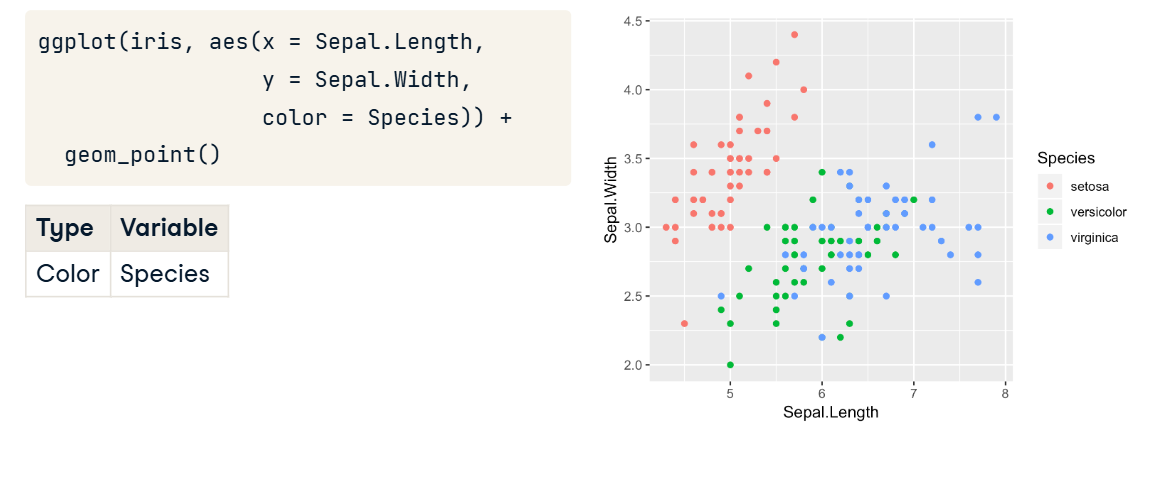
\includegraphics{../images/im136.png}
\end{frame}

\begin{frame}{Mapping onto the color aesthetic}
\phantomsection\label{mapping-onto-the-color-aesthetic}
That is, we map a variable from our dataframe onto one of the visible
aesthetics.

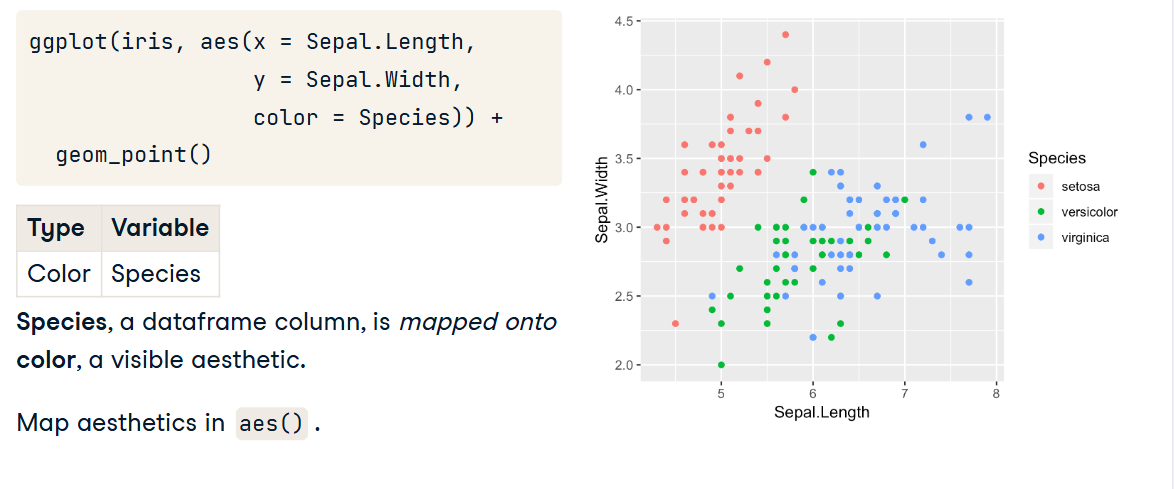
\includegraphics{../images/im137.png} We call a column in our dataframe
to be mapped onto a visible aesthetic.
\end{frame}

\begin{frame}{Mapping onto the color aesthetic}
\phantomsection\label{mapping-onto-the-color-aesthetic-1}
That's why we made such a big deal about data structure earlier.

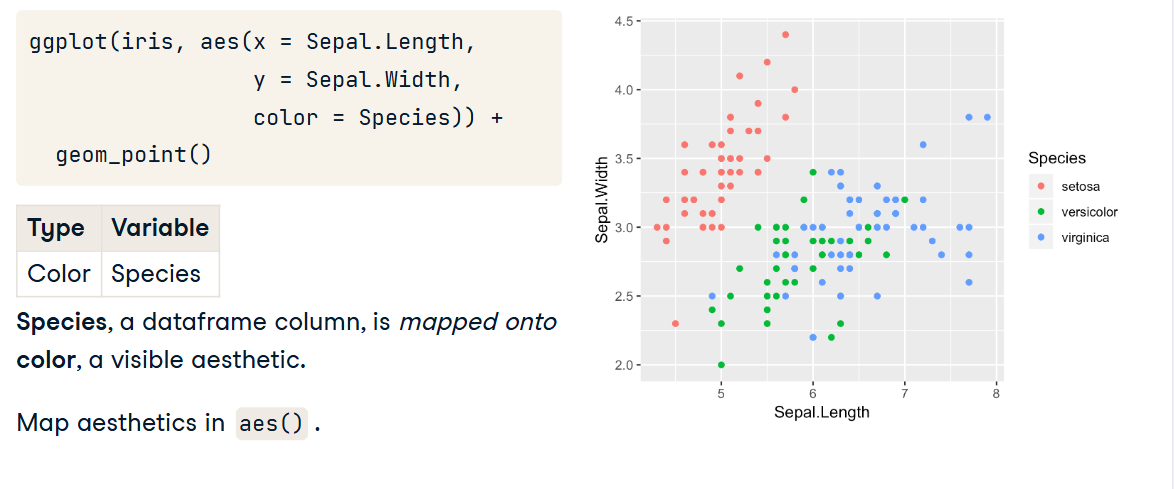
\includegraphics{../images/im137.png}

Each mapped variable is its own column variable in the data frame.
\end{frame}

\begin{frame}{Mapping onto the color aesthetic in geom}
\phantomsection\label{mapping-onto-the-color-aesthetic-in-geom}
Importantly, we call aesthetics in the aes function. We could have also
called aesthetics in the geom layer as shown here, and get the same
result.

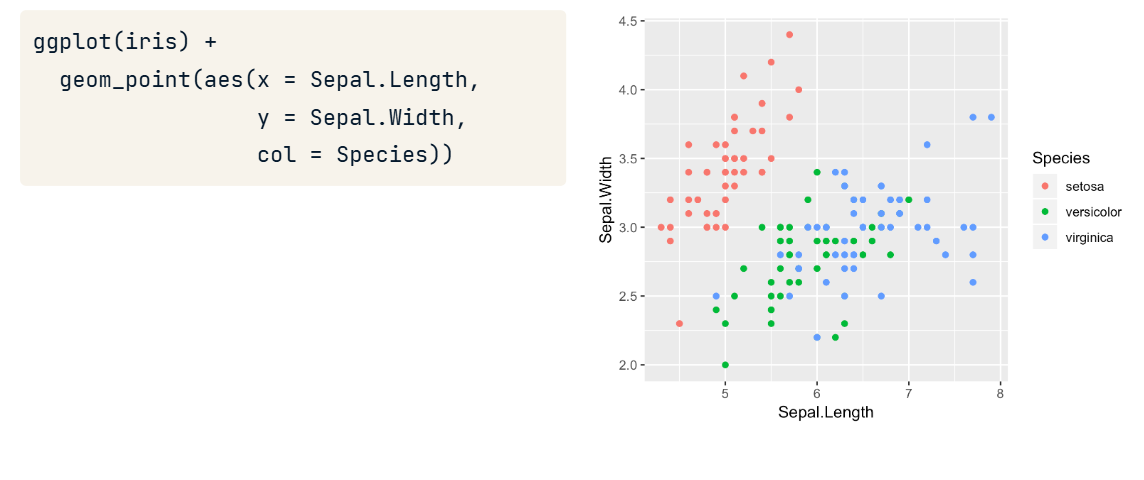
\includegraphics{../images/im138.png} \#\# Mapping onto the color
aesthetic in geom

\begin{itemize}
\item
  This is typically only done if we don't want all layers to inherit the
  same aesthetics or we're mixing different data sources.
\item
  In general, try to keep your data and aesthetics layer in the same
  ggplot function definition.
\end{itemize}
\end{frame}

\begin{frame}{Typical visible aesthetics}
\phantomsection\label{typical-visible-aesthetics}
In addition to the X and Y axes and color, typical visible aesthetics
include

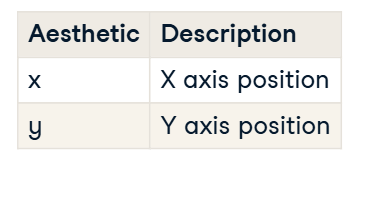
\includegraphics{../images/im139.png}
\end{frame}

\begin{frame}{Typical visible aesthetics}
\phantomsection\label{typical-visible-aesthetics-1}
fill, which is distinct from

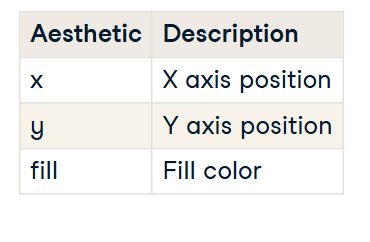
\includegraphics{../images/im140.png}
\end{frame}

\begin{frame}{Typical visible aesthetics}
\phantomsection\label{typical-visible-aesthetics-2}
color in that color usually, but not always, refers to the outline of a
shape.

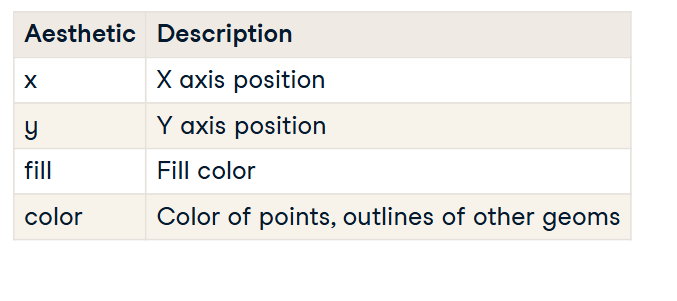
\includegraphics{../images/im141.png}
\end{frame}

\begin{frame}{Typical visible aesthetics}
\phantomsection\label{typical-visible-aesthetics-3}
Size adjusts the area or radius of points, the thickness of lines and
the font size of text.

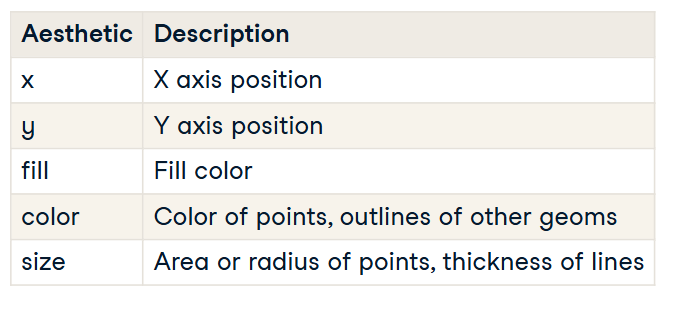
\includegraphics{../images/im142.png}
\end{frame}

\begin{frame}{Typical visible aesthetics}
\phantomsection\label{typical-visible-aesthetics-4}
alpha refers to alpha-blending, which adjusts the transparency of a
shape.

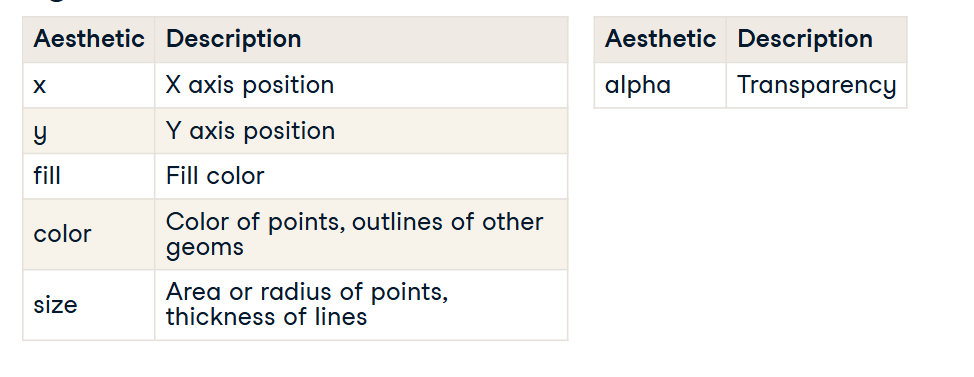
\includegraphics{../images/im143.png}
\end{frame}

\begin{frame}{Typical visible aesthetics}
\phantomsection\label{typical-visible-aesthetics-5}
line type refers to the dash pattern of a line and

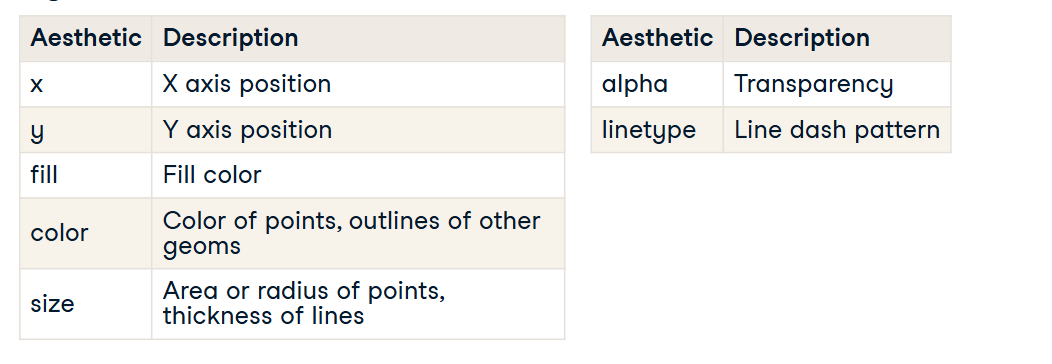
\includegraphics{../images/im144.png}
\end{frame}

\begin{frame}{Typical visible aesthetics}
\phantomsection\label{typical-visible-aesthetics-6}
labels are direct labels of an item, directly on the plot. Like printing
an item's name on a scatter plot instead of just drawing a point.

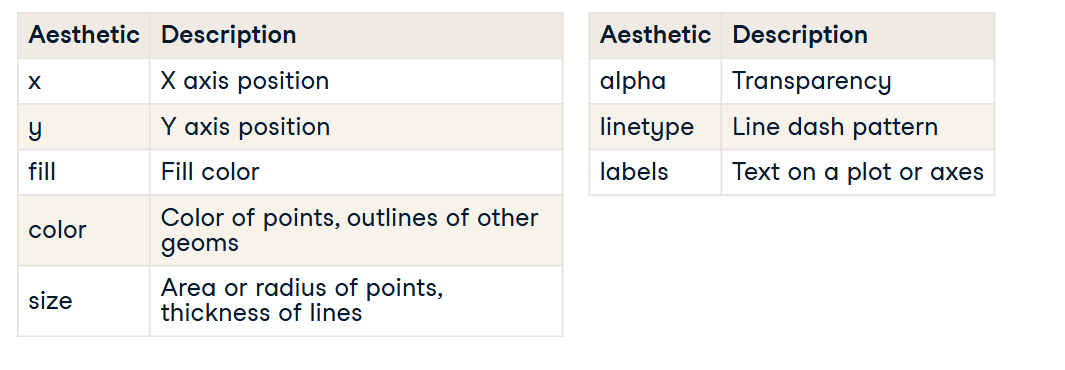
\includegraphics{../images/im145.png}
\end{frame}

\begin{frame}{Typical visible aesthetics}
\phantomsection\label{typical-visible-aesthetics-7}
Direct labeling of points is an extension of axis labels for categorical
data in that they are unambiguous, and
\end{frame}

\begin{frame}{Typical visible aesthetics}
\phantomsection\label{typical-visible-aesthetics-8}
Shape refers to the shape of a point.

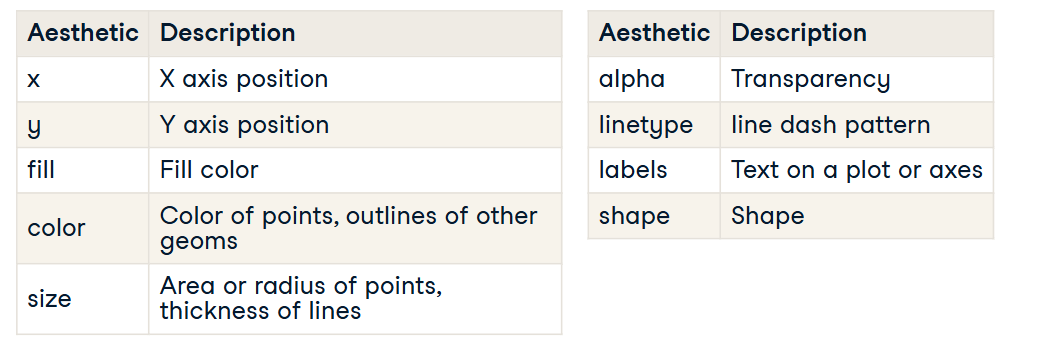
\includegraphics{../images/im146.png}
\end{frame}

\begin{frame}{Typical visible aesthetics}
\phantomsection\label{typical-visible-aesthetics-9}
Many of these aesthetics function as both aesthetic mappings as well as
attributes, and one of the most common mistakes beginners make is
confusing the two or overwriting aesthetic mappings with fixed
attributes.
\end{frame}

\begin{frame}{Typical visible aesthetics}
\phantomsection\label{typical-visible-aesthetics-10}
Our goal here is to not only show you how to use them correctly but
appropriately for the plot's type and purpose.
\end{frame}

\begin{frame}{Typical visible aesthetics}
\phantomsection\label{typical-visible-aesthetics-11}
Just like our two main variable types, there are visible aesthetics for
continuous and categorical data which we'll explore in the next video,
\end{frame}

\begin{frame}[fragile]{Practice 1: Introduction to Aesthetics in
ggplot2}
\phantomsection\label{practice-1-introduction-to-aesthetics-in-ggplot2}
\begin{itemize}
\tightlist
\item
  Aesthetics are visual properties that can be mapped to data variables.
\item
  Examples include \texttt{x}, \texttt{y}, \texttt{color},
  \texttt{size}, and \texttt{shape}.
\end{itemize}
\end{frame}

\begin{frame}[fragile]{Practice 1: Map Variables to Aesthetics}
\phantomsection\label{practice-1-map-variables-to-aesthetics}
\begin{itemize}
\tightlist
\item
  \textbf{Objective}: Map \texttt{mpg} to the x-axis and \texttt{cyl} to
  the y-axis.
\item
  Use \texttt{aes()} to define mappings.
\end{itemize}
\end{frame}

\begin{frame}[fragile]{Practice 1:}
\phantomsection\label{practice-1}
\AddToHookNext{env/Highlighting/begin}{\tiny}

\begin{Shaded}
\begin{Highlighting}[]
\CommentTok{\# Load ggplot2 package}
\FunctionTok{library}\NormalTok{(ggplot2)}
\CommentTok{\# Map mpg to x and cyl to y}
\FunctionTok{ggplot}\NormalTok{(mtcars, }\FunctionTok{aes}\NormalTok{(}\AttributeTok{x =}\NormalTok{ mpg, }\AttributeTok{y =}\NormalTok{ cyl)) }\SpecialCharTok{+} \FunctionTok{geom\_point}\NormalTok{()}
\end{Highlighting}
\end{Shaded}

\begin{center}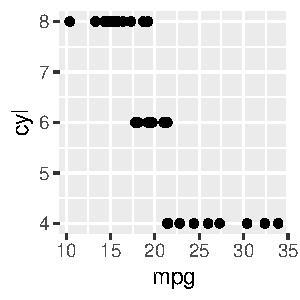
\includegraphics[width=0.5\linewidth]{Figs/unnamed-chunk-10-1} \end{center}
\end{frame}

\begin{frame}[fragile]{Practice 1: Swap Aesthetic Mappings}
\phantomsection\label{practice-1-swap-aesthetic-mappings}
Objective: Map cyl to the x-axis and mpg to the y-axis.

\AddToHookNext{env/Highlighting/begin}{\tiny}

\begin{Shaded}
\begin{Highlighting}[]
\CommentTok{\# Swap x and y aesthetics}
\FunctionTok{ggplot}\NormalTok{(mtcars, }\FunctionTok{aes}\NormalTok{(}\AttributeTok{x =}\NormalTok{ cyl, }\AttributeTok{y =}\NormalTok{ mpg)) }\SpecialCharTok{+} \FunctionTok{geom\_point}\NormalTok{()}
\end{Highlighting}
\end{Shaded}

\begin{center}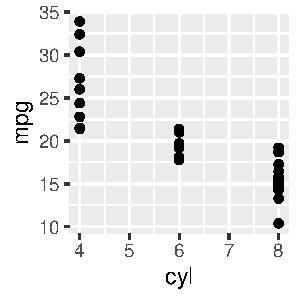
\includegraphics[width=0.5\linewidth]{Figs/unnamed-chunk-11-1} \end{center}
\end{frame}

\begin{frame}[fragile]{Practice 1: Add More Aesthetics}
\phantomsection\label{practice-1-add-more-aesthetics}
Objective: Map wt to x, mpg to y, and cyl to color.

\AddToHookNext{env/Highlighting/begin}{\tiny}

\begin{Shaded}
\begin{Highlighting}[]
\CommentTok{\# Add more aesthetics: color}
\FunctionTok{ggplot}\NormalTok{(mtcars, }\FunctionTok{aes}\NormalTok{(}\AttributeTok{x =}\NormalTok{ wt, }\AttributeTok{y =}\NormalTok{ mpg, }\AttributeTok{color =}\NormalTok{ cyl)) }\SpecialCharTok{+} \FunctionTok{geom\_point}\NormalTok{()}
\end{Highlighting}
\end{Shaded}

\begin{center}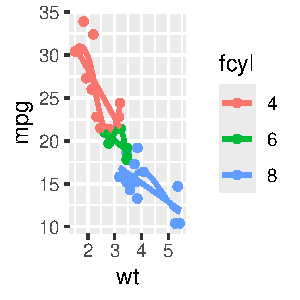
\includegraphics[width=0.5\linewidth]{Figs/unnamed-chunk-12-1} \end{center}
\end{frame}

\begin{frame}[fragile]{Practice 1: Customize Shape and Size}
\phantomsection\label{practice-1-customize-shape-and-size}
Objective: Modify the plot by changing shape to 1 and increasing size to
4.

\AddToHookNext{env/Highlighting/begin}{\tiny}

\begin{Shaded}
\begin{Highlighting}[]
\CommentTok{\# Customize shape and size}
\FunctionTok{ggplot}\NormalTok{(mtcars, }\FunctionTok{aes}\NormalTok{(}\AttributeTok{x =}\NormalTok{ wt, }\AttributeTok{y =}\NormalTok{ mpg, }\AttributeTok{color =}\NormalTok{ cyl)) }\SpecialCharTok{+} \FunctionTok{geom\_point}\NormalTok{(}\AttributeTok{shape =} \DecValTok{1}\NormalTok{,}
    \AttributeTok{size =} \DecValTok{4}\NormalTok{)}
\end{Highlighting}
\end{Shaded}

\begin{center}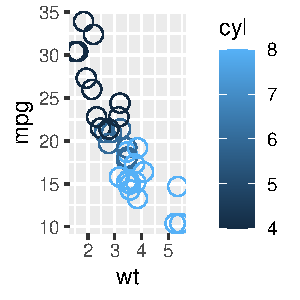
\includegraphics[width=0.5\linewidth]{Figs/unnamed-chunk-13-1} \end{center}
\end{frame}

\begin{frame}[fragile]{Understanding Color and Fill in ggplot2}
\phantomsection\label{understanding-color-and-fill-in-ggplot2}
\begin{itemize}
\tightlist
\item
  The \texttt{color} aesthetic changes the \textbf{outline} of a
  geometry.
\item
  The \texttt{fill} aesthetic changes the \textbf{inside} of a geometry.
\item
  Certain shapes allow both \texttt{color} and \texttt{fill} to be
  mapped.
\end{itemize}
\end{frame}

\begin{frame}[fragile]{Practice 2: Map \texttt{cyl} to \texttt{fill}}
\phantomsection\label{practice-2-map-cyl-to-fill}
\begin{itemize}
\tightlist
\item
  \textbf{Objective}: Map \texttt{wt} to the x-axis, \texttt{mpg} to the
  y-axis, and \texttt{cyl} to the \texttt{fill} aesthetic.
\end{itemize}
\end{frame}

\begin{frame}[fragile]{Practice 2: Map \texttt{cyl} to \texttt{fill}}
\phantomsection\label{practice-2-map-cyl-to-fill-1}
\AddToHookNext{env/Highlighting/begin}{\tiny}

\begin{Shaded}
\begin{Highlighting}[]
\CommentTok{\# Load ggplot2 package}
\FunctionTok{library}\NormalTok{(ggplot2)}

\CommentTok{\# Map cyl to fill}
\FunctionTok{ggplot}\NormalTok{(mtcars, }\FunctionTok{aes}\NormalTok{(}\AttributeTok{x =}\NormalTok{ wt, }\AttributeTok{y =}\NormalTok{ mpg, }\AttributeTok{fill =}\NormalTok{ cyl)) }\SpecialCharTok{+} \FunctionTok{geom\_point}\NormalTok{(}\AttributeTok{shape =} \DecValTok{21}\NormalTok{,}
    \AttributeTok{size =} \DecValTok{4}\NormalTok{)}
\end{Highlighting}
\end{Shaded}

\begin{center}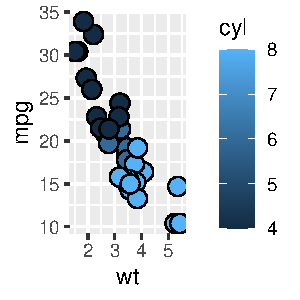
\includegraphics[width=0.5\linewidth]{Figs/unnamed-chunk-14-1} \end{center}
\end{frame}

\begin{frame}{Practice 2: Customize Shape and Transparency}
\phantomsection\label{practice-2-customize-shape-and-transparency}
\begin{itemize}
\item
  Objective: Use shape = 21 to allow both fill and color mapping.
\item
  Add alpha = 0.6 for partial transparency.
\end{itemize}
\end{frame}

\begin{frame}[fragile]{Practice 2: Customize Shape and Transparency}
\phantomsection\label{practice-2-customize-shape-and-transparency-1}
\AddToHookNext{env/Highlighting/begin}{\tiny}

\begin{Shaded}
\begin{Highlighting}[]
\CommentTok{\# Customize shape and transparency}
\FunctionTok{ggplot}\NormalTok{(mtcars, }\FunctionTok{aes}\NormalTok{(}\AttributeTok{x =}\NormalTok{ wt, }\AttributeTok{y =}\NormalTok{ mpg, }\AttributeTok{fill =}\NormalTok{ cyl)) }\SpecialCharTok{+} \FunctionTok{geom\_point}\NormalTok{(}\AttributeTok{shape =} \DecValTok{21}\NormalTok{,}
    \AttributeTok{size =} \DecValTok{4}\NormalTok{, }\AttributeTok{alpha =} \FloatTok{0.6}\NormalTok{)}
\end{Highlighting}
\end{Shaded}

\begin{center}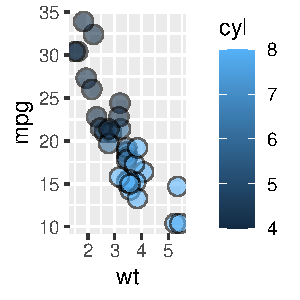
\includegraphics[width=0.5\linewidth]{Figs/unnamed-chunk-15-1} \end{center}
\end{frame}

\begin{frame}[fragile]{Practice 3: Map gear to color}
\phantomsection\label{practice-3-map-gear-to-color}
Objective: Add gear as a color aesthetic for outlines.

\AddToHookNext{env/Highlighting/begin}{\tiny}

\begin{Shaded}
\begin{Highlighting}[]
\CommentTok{\# Map gear to color}
\FunctionTok{ggplot}\NormalTok{(mtcars, }\FunctionTok{aes}\NormalTok{(}\AttributeTok{x =}\NormalTok{ wt, }\AttributeTok{y =}\NormalTok{ mpg, }\AttributeTok{fill =}\NormalTok{ cyl, }\AttributeTok{color =}\NormalTok{ gear)) }\SpecialCharTok{+}
    \FunctionTok{geom\_point}\NormalTok{(}\AttributeTok{shape =} \DecValTok{21}\NormalTok{, }\AttributeTok{size =} \DecValTok{4}\NormalTok{, }\AttributeTok{alpha =} \FloatTok{0.6}\NormalTok{)}
\end{Highlighting}
\end{Shaded}

\begin{center}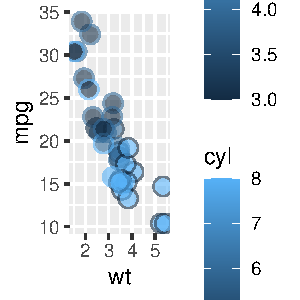
\includegraphics[width=0.5\linewidth]{Figs/unnamed-chunk-16-1} \end{center}
\end{frame}

\begin{frame}{Practice 4: Comparing Aesthetics in ggplot2}
\phantomsection\label{practice-4-comparing-aesthetics-in-ggplot2}
\begin{itemize}
\tightlist
\item
  ggplot2 aesthetics control visual elements like size, shape, alpha,
  and labels.
\item
  Care must be taken to avoid overriding aesthetics unintentionally.
\end{itemize}
\end{frame}

\begin{frame}[fragile]{Practice 4: Base Plot with Size Mapping}
\phantomsection\label{practice-4-base-plot-with-size-mapping}
\begin{itemize}
\tightlist
\item
  \textbf{Objective}: Create a base plot and map \texttt{cyl} to the
  \texttt{size} aesthetic.
\end{itemize}

\begin{Shaded}
\begin{Highlighting}[]
\CommentTok{\# Establish the base layer}
\NormalTok{plt\_mpg\_vs\_wt }\OtherTok{\textless{}{-}} \FunctionTok{ggplot}\NormalTok{(mtcars, }\FunctionTok{aes}\NormalTok{(}\AttributeTok{x =}\NormalTok{ wt, }\AttributeTok{y =}\NormalTok{ mpg))}

\CommentTok{\# Map cyl to size}
\NormalTok{plt\_mpg\_vs\_wt }\SpecialCharTok{+} \FunctionTok{geom\_point}\NormalTok{(}\FunctionTok{aes}\NormalTok{(}\AttributeTok{size =}\NormalTok{ cyl))}
\end{Highlighting}
\end{Shaded}

\begin{center}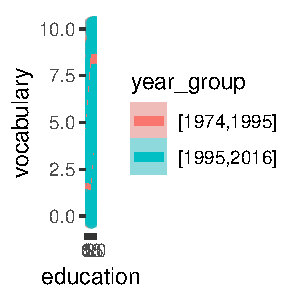
\includegraphics[width=0.5\linewidth]{Figs/unnamed-chunk-17-1} \end{center}
\end{frame}

\begin{frame}[fragile]{Practice 4: Map cyl to Alpha}
\phantomsection\label{practice-4-map-cyl-to-alpha}
Objective: Map the cyl variable to the alpha aesthetic.

\begin{Shaded}
\begin{Highlighting}[]
\CommentTok{\# Map cyl to alpha}
\NormalTok{plt\_mpg\_vs\_wt }\SpecialCharTok{+} \FunctionTok{geom\_point}\NormalTok{(}\FunctionTok{aes}\NormalTok{(}\AttributeTok{alpha =}\NormalTok{ cyl))}
\end{Highlighting}
\end{Shaded}

\begin{center}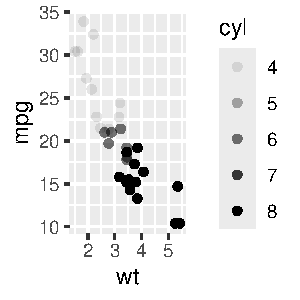
\includegraphics[width=0.5\linewidth]{Figs/unnamed-chunk-18-1} \end{center}
\end{frame}

\begin{frame}[fragile]{Practice 4: Map cyl to Shape}
\phantomsection\label{practice-4-map-cyl-to-shape}
Objective: Map cyl to the shape aesthetic.

\begin{Shaded}
\begin{Highlighting}[]
\CommentTok{\# Map cyl to shape}
\NormalTok{plt\_mpg\_vs\_wt }\SpecialCharTok{+} \FunctionTok{geom\_point}\NormalTok{(}\FunctionTok{aes}\NormalTok{(}\AttributeTok{shape =} \FunctionTok{factor}\NormalTok{(cyl)))}
\end{Highlighting}
\end{Shaded}

\begin{center}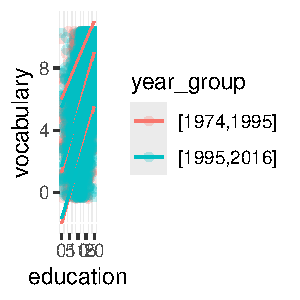
\includegraphics[width=0.5\linewidth]{Figs/unnamed-chunk-19-1} \end{center}
\end{frame}

\begin{frame}[fragile]{Practice 4: Map cyl to Label}
\phantomsection\label{practice-4-map-cyl-to-label}
Objective: Map cyl to the label aesthetic and switch to geom\_text().

\begin{Shaded}
\begin{Highlighting}[]
\CommentTok{\# Map cyl to label and use geom\_text}
\NormalTok{plt\_mpg\_vs\_wt }\SpecialCharTok{+} \FunctionTok{geom\_text}\NormalTok{(}\FunctionTok{aes}\NormalTok{(}\AttributeTok{label =}\NormalTok{ cyl))}
\end{Highlighting}
\end{Shaded}

\begin{center}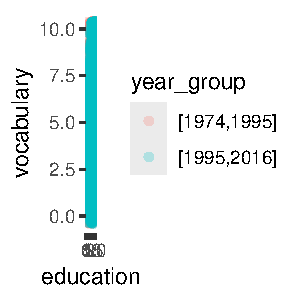
\includegraphics[width=0.5\linewidth]{Figs/unnamed-chunk-20-1} \end{center}
\end{frame}

\begin{frame}{Using attributes}
\phantomsection\label{using-attributes}
\begin{itemize}
\item
  In the last exercises you learned a fundamental concept of ggplot2:
  aesthetic mappings.
\item
  Colloquially, when we say aesthetics we're describing how something
  looks, but now you know that in ggplot2, we're talking about aesthetic
  mappings.
\end{itemize}
\end{frame}

\begin{frame}{Using attributes}
\phantomsection\label{using-attributes-1}
\begin{itemize}
\item
  If we talk about how something looks, we refer to its attributes.
\item
  One of the most confusing parts of ggplot2 is that all our visible
  aesthetics also exist as attributes.
\end{itemize}
\end{frame}

\begin{frame}{Aesthetics? Attributes!}
\phantomsection\label{aesthetics-attributes}
so it's easy to mix up the two! Attributes are always called in the geom
layer (which we'll discuss in more detail in the next part).

\includegraphics{../images/im147.png}

For example, to change the color of these points to red, we'd just set
the plot's attribute using the color argument in the geom layer.
\end{frame}

\begin{frame}{Aesthetics? Attributes!}
\phantomsection\label{aesthetics-attributes-1}
For example, it's color attribute is set by the color argument, its size
by the size argument

\includegraphics{../images/im149.png}
\end{frame}

\begin{frame}{Aesthetics? Attributes!}
\phantomsection\label{aesthetics-attributes-2}
and its shape by the shape argument.

\includegraphics{../images/im150.png}

The distinction between aesthetics and attributes is subtle but
important. Mixing the two is a very common mistake.
\end{frame}

\begin{frame}[fragile]{Practice 1: Set Color and Alpha}
\phantomsection\label{practice-1-set-color-and-alpha}
\begin{itemize}
\tightlist
\item
  Use fixed values for the point \texttt{color} and \texttt{alpha}.
\end{itemize}

\AddToHookNext{env/Highlighting/begin}{\tiny}

\begin{Shaded}
\begin{Highlighting}[]
\CommentTok{\# Define a hexadecimal color}
\NormalTok{my\_blue }\OtherTok{\textless{}{-}} \StringTok{"\#4ABEFF"}

\CommentTok{\# Create a plot with fixed color and transparency}
\FunctionTok{ggplot}\NormalTok{(mtcars, }\FunctionTok{aes}\NormalTok{(}\AttributeTok{x =}\NormalTok{ wt, }\AttributeTok{y =}\NormalTok{ mpg)) }\SpecialCharTok{+} \FunctionTok{geom\_point}\NormalTok{(}\AttributeTok{color =}\NormalTok{ my\_blue,}
    \AttributeTok{alpha =} \FloatTok{0.6}\NormalTok{)}
\end{Highlighting}
\end{Shaded}

\begin{center}\includegraphics[width=0.5\linewidth]{Figs/unnamed-chunk-21-1} \end{center}
\end{frame}

\begin{frame}[fragile]{Practice 1: Conflicts Between Attributes and
Aesthetics}
\phantomsection\label{practice-1-conflicts-between-attributes-and-aesthetics}
Transparency can be controlled using alpha.

\AddToHookNext{env/Highlighting/begin}{\tiny}

\begin{Shaded}
\begin{Highlighting}[]
\CommentTok{\# Add a point layer with alpha transparency}
\FunctionTok{ggplot}\NormalTok{(mtcars, }\FunctionTok{aes}\NormalTok{(}\AttributeTok{x =}\NormalTok{ wt, }\AttributeTok{y =}\NormalTok{ mpg, }\AttributeTok{color =}\NormalTok{ cyl)) }\SpecialCharTok{+} \FunctionTok{geom\_point}\NormalTok{(}\AttributeTok{alpha =} \FloatTok{0.5}\NormalTok{)}
\end{Highlighting}
\end{Shaded}

\begin{center}\includegraphics[width=0.5\linewidth]{Figs/unnamed-chunk-22-1} \end{center}
\end{frame}

\begin{frame}[fragile]{Practice 1: Add Labels to Points}
\phantomsection\label{practice-1-add-labels-to-points}
Use geom\_text() to label points with the row names.

\AddToHookNext{env/Highlighting/begin}{\tiny}

\begin{Shaded}
\begin{Highlighting}[]
\CommentTok{\# Add text labels}
\FunctionTok{ggplot}\NormalTok{(mtcars, }\FunctionTok{aes}\NormalTok{(}\AttributeTok{x =}\NormalTok{ wt, }\AttributeTok{y =}\NormalTok{ mpg)) }\SpecialCharTok{+} \FunctionTok{geom\_text}\NormalTok{(}\FunctionTok{aes}\NormalTok{(}\AttributeTok{label =} \FunctionTok{rownames}\NormalTok{(mtcars)),}
    \AttributeTok{color =} \StringTok{"red"}\NormalTok{)}
\end{Highlighting}
\end{Shaded}

\begin{center}\includegraphics[width=0.5\linewidth]{Figs/unnamed-chunk-23-1} \end{center}
\end{frame}

\begin{frame}[fragile]{Practice 1: Customize Shape and Color}
\phantomsection\label{practice-1-customize-shape-and-color}
Change the shape and color of points.

\AddToHookNext{env/Highlighting/begin}{\tiny}

\begin{Shaded}
\begin{Highlighting}[]
\CommentTok{\# Customize points with shape and color}
\FunctionTok{ggplot}\NormalTok{(mtcars, }\FunctionTok{aes}\NormalTok{(}\AttributeTok{x =}\NormalTok{ wt, }\AttributeTok{y =}\NormalTok{ mpg)) }\SpecialCharTok{+} \FunctionTok{geom\_point}\NormalTok{(}\AttributeTok{shape =} \DecValTok{24}\NormalTok{,}
    \AttributeTok{color =} \StringTok{"yellow"}\NormalTok{)}
\end{Highlighting}
\end{Shaded}

\begin{center}\includegraphics[width=0.5\linewidth]{Figs/unnamed-chunk-24-1} \end{center}
\end{frame}

\begin{frame}[fragile]{Practice 1: Complex Aesthetic Mapping}
\phantomsection\label{practice-1-complex-aesthetic-mapping}
Map qsec to the y-axis, mpg to the x-axis, and cyl to color.

\AddToHookNext{env/Highlighting/begin}{\tiny}

\begin{Shaded}
\begin{Highlighting}[]
\CommentTok{\# Map multiple aesthetics}
\FunctionTok{ggplot}\NormalTok{(mtcars, }\FunctionTok{aes}\NormalTok{(}\AttributeTok{x =}\NormalTok{ mpg, }\AttributeTok{y =}\NormalTok{ qsec, }\AttributeTok{color =}\NormalTok{ cyl)) }\SpecialCharTok{+} \FunctionTok{geom\_point}\NormalTok{()}
\end{Highlighting}
\end{Shaded}

\begin{center}\includegraphics[width=0.5\linewidth]{Figs/unnamed-chunk-25-1} \end{center}
\end{frame}

\begin{frame}[fragile]{Practice 1: Add More Aesthetics}
\phantomsection\label{practice-1-add-more-aesthetics-1}
Map gear (factor version of am) to shape.

\AddToHookNext{env/Highlighting/begin}{\tiny}

\begin{Shaded}
\begin{Highlighting}[]
\CommentTok{\# Add shape mapping}
\FunctionTok{ggplot}\NormalTok{(mtcars, }\FunctionTok{aes}\NormalTok{(}\AttributeTok{x =}\NormalTok{ mpg, }\AttributeTok{y =}\NormalTok{ qsec, }\AttributeTok{color =}\NormalTok{ cyl, }\AttributeTok{shape =} \FunctionTok{factor}\NormalTok{(gear))) }\SpecialCharTok{+}
    \FunctionTok{geom\_point}\NormalTok{()}
\end{Highlighting}
\end{Shaded}

\begin{center}\includegraphics[width=0.5\linewidth]{Figs/unnamed-chunk-26-1} \end{center}
\end{frame}

\begin{frame}[fragile]{Practice 1: Map to Size}
\phantomsection\label{practice-1-map-to-size}
Map hp divided by wt to size.

\AddToHookNext{env/Highlighting/begin}{\tiny}

\begin{Shaded}
\begin{Highlighting}[]
\CommentTok{\# Add size mapping}
\FunctionTok{ggplot}\NormalTok{(mtcars, }\FunctionTok{aes}\NormalTok{(}\AttributeTok{x =}\NormalTok{ mpg, }\AttributeTok{y =}\NormalTok{ qsec, }\AttributeTok{color =}\NormalTok{ cyl, }\AttributeTok{shape =} \FunctionTok{factor}\NormalTok{(gear),}
    \AttributeTok{size =}\NormalTok{ hp}\SpecialCharTok{/}\NormalTok{wt)) }\SpecialCharTok{+} \FunctionTok{geom\_point}\NormalTok{()}
\end{Highlighting}
\end{Shaded}

\begin{center}\includegraphics[width=0.5\linewidth]{Figs/unnamed-chunk-27-1} \end{center}
\end{frame}

\begin{frame}{Modifying Aesthetics}
\phantomsection\label{modifying-aesthetics}
Now that we know what aesthetics are and have some idea about choosing
them appropriately, let's explore how to modify them.
\end{frame}

\begin{frame}{Positions}
\phantomsection\label{positions}
A common adjustment is the position.

\includegraphics{../images/im152.png}
\end{frame}

\begin{frame}{Positions}
\phantomsection\label{positions-1}
\begin{itemize}
\item
  Position specifies how ggplot will adjust for overlapping bars or
  points on a single layer.
\item
  For example, we have identity, dodge, stack, fill, jitter,
  jitterdodge, and nudge. Let's take a look.
\end{itemize}
\end{frame}

\begin{frame}{position = ``identity'' (default)}
\phantomsection\label{position-identity-default}
The most straightforward position is identity, which we've actually
already seen.

\includegraphics{../images/im153.png}

It's the default position for our scatter plots.
\end{frame}

\begin{frame}{position = ``identity'' (default)}
\phantomsection\label{position-identity-default-1}
``Identity'' means that the value in the data frame is exactly where the
value will be positioned in the plot.

\includegraphics{../images/im153.png}

This basically means, don't do anything, just put the information where
the data says to put the information.
\end{frame}

\begin{frame}{position = ``identity'' (default)}
\phantomsection\label{position-identity-default-2}
We could have written it explicitly, but it's not necessary.

\includegraphics{../images/im154.png}

There is an issue with the precision in this data set.
\end{frame}

\begin{frame}{position = ``identity'' (default)}
\phantomsection\label{position-identity-default-3}
Our sepals were measured to the nearest millimeter. So although we only
have 150 points, there is too much overplotting to distinguish them.

To solve this, we need to add some random noise on both the x and y axes
to see regions of high density - which is referred to as ``jittering''.
\end{frame}

\begin{frame}{position = ``jitter''}
\phantomsection\label{position-jitter}
``jitter'' can be used as an argument, but each position type can also
be accessed as a function. For example,

\includegraphics{../images/im155.png}
\end{frame}

\begin{frame}{position\_jitter()}
\phantomsection\label{position_jitter}
position jitter can be defined in a function before we call our plot, as
shown here.

\includegraphics{../images/im156.png}

This has two advantages.
\end{frame}

\begin{frame}{position\_jitter()}
\phantomsection\label{position_jitter-1}
Now we can set specific arguments for the position, such as the width,
which defines how much random noise should be added, and it allows us to
use this parameter throughout our plotting functions so that we can
maintain consistency across plots.

\includegraphics{../images/im157.png}

This is available for all position attributes. We'll explore the other
positions in the exercises.
\end{frame}

\begin{frame}{Scale functions}
\phantomsection\label{scale-functions}
\begin{itemize}
\tightlist
\item
  Recall that each of the aesthetics is a scale which we mapped data
  onto, so color is just a scale, like x and y are scales.
\end{itemize}

\includegraphics{../images/im158.png}
\end{frame}

\begin{frame}{Scale functions}
\phantomsection\label{scale-functions-1}
Appropriately enough, we can access all the scales with the scale
underscore functions.

\includegraphics{../images/im159.png}\\
The second part of the function defines which scale we want to modify.
\end{frame}

\begin{frame}{Scale functions}
\phantomsection\label{scale-functions-2}
All the aesthetics we saw earlier have an associated scale function.

\includegraphics{../images/im159.png}

The third part must match the type of data we are using. Here discrete
means we are working with categorical data.
\end{frame}

\begin{frame}{Scale functions}
\phantomsection\label{scale-functions-3}
That means we have to choose our axis dependent on the type of data we
have.

\includegraphics{../images/im159.png}

Here, we'll consider the continuous x aesthetic and the categorical
color aesthetic.
\end{frame}

\begin{frame}{Scale functions}
\phantomsection\label{scale-functions-4}
Just as an aside, before we move on - don't let the naming conventions
confuse you.

\includegraphics{../images/im159.png}

Categorical variables are also called factors, discrete and qualitative
depending on their context and who you're talking to.
\end{frame}

\begin{frame}{scale\_*\_*()}
\phantomsection\label{scale__}
There are many arguments for the scale functions.

\includegraphics{../images/im160.png}

The first argument is always the name of the scale, after that most
common are limits, breaks, expand and labels.
\end{frame}

\begin{frame}{The limits argument}
\phantomsection\label{the-limits-argument}
limits describe the scale's range.

\includegraphics{../images/im161.png}
\end{frame}

\begin{frame}{The breaks argument}
\phantomsection\label{the-breaks-argument}
breaks control the tick mark positions.

\includegraphics{../images/im162.png}
\end{frame}

\begin{frame}{The expand argument}
\phantomsection\label{the-expand-argument}
expand is a numeric vector of length two, giving a multiplicative and
additive constant used to expand the range of the scales so that there
is a small gap between the data and the axes.

\includegraphics{../images/im163.png}
\end{frame}

\begin{frame}{The labels argument}
\phantomsection\label{the-labels-argument}
and labels adjust the category names.

\includegraphics{../images/im164.png}
\end{frame}

\begin{frame}{labs()}
\phantomsection\label{labs}
Note that if we just want to quickly change the axis labels, we can do
this with the labs function.

\includegraphics{../images/im165.png}
\end{frame}

\begin{frame}{Practice 1: Updating Aesthetic Labels}
\phantomsection\label{practice-1-updating-aesthetic-labels}
\end{frame}

\begin{frame}[fragile]{Step 1: Add Axis Labels}
\phantomsection\label{step-1-add-axis-labels}
\begin{itemize}
\tightlist
\item
  Use the \texttt{labs()} function to set x and y-axis labels.
\end{itemize}

\AddToHookNext{env/Highlighting/begin}{\tiny}

\begin{Shaded}
\begin{Highlighting}[]
\NormalTok{palette }\OtherTok{\textless{}{-}} \FunctionTok{c}\NormalTok{(}\AttributeTok{automatic =} \StringTok{"\#377EB8"}\NormalTok{, }\AttributeTok{manual =} \StringTok{"\#E41A1C"}\NormalTok{)}

\FunctionTok{ggplot}\NormalTok{(mtcars, }\FunctionTok{aes}\NormalTok{(}\AttributeTok{x =}\NormalTok{ cyl, }\AttributeTok{fill =} \FunctionTok{factor}\NormalTok{(gear))) }\SpecialCharTok{+} \FunctionTok{geom\_bar}\NormalTok{() }\SpecialCharTok{+}
    \FunctionTok{labs}\NormalTok{(}\AttributeTok{x =} \StringTok{"Number of Cylinders"}\NormalTok{, }\AttributeTok{y =} \StringTok{"Count"}\NormalTok{, }\AttributeTok{fill =} \StringTok{"Gear"}\NormalTok{)}
\end{Highlighting}
\end{Shaded}

\begin{center}\includegraphics[width=0.5\linewidth]{Figs/unnamed-chunk-28-1} \end{center}
\end{frame}

\begin{frame}[fragile]{Step 2: Customize Fill Colors}
\phantomsection\label{step-2-customize-fill-colors}
Use scale\_fill\_manual() to define custom colors and a legend title.

\AddToHookNext{env/Highlighting/begin}{\tiny}

\begin{Shaded}
\begin{Highlighting}[]
\CommentTok{\# Define custom colors for gear levels}
\NormalTok{palette }\OtherTok{\textless{}{-}} \FunctionTok{c}\NormalTok{(}\StringTok{\textasciigrave{}}\AttributeTok{3}\StringTok{\textasciigrave{}} \OtherTok{=} \StringTok{"\#377EB8"}\NormalTok{, }\StringTok{\textasciigrave{}}\AttributeTok{4}\StringTok{\textasciigrave{}} \OtherTok{=} \StringTok{"\#E41A1C"}\NormalTok{, }\StringTok{\textasciigrave{}}\AttributeTok{5}\StringTok{\textasciigrave{}} \OtherTok{=} \StringTok{"\#4DAF4A"}\NormalTok{)}

\FunctionTok{ggplot}\NormalTok{(mtcars, }\FunctionTok{aes}\NormalTok{(}\AttributeTok{x =}\NormalTok{ cyl, }\AttributeTok{fill =} \FunctionTok{factor}\NormalTok{(gear))) }\SpecialCharTok{+} \FunctionTok{geom\_bar}\NormalTok{() }\SpecialCharTok{+}
    \FunctionTok{labs}\NormalTok{(}\AttributeTok{x =} \StringTok{"Number of Cylinders"}\NormalTok{, }\AttributeTok{y =} \StringTok{"Count"}\NormalTok{, }\AttributeTok{fill =} \StringTok{"Gear"}\NormalTok{) }\SpecialCharTok{+}
    \FunctionTok{scale\_fill\_manual}\NormalTok{(}\AttributeTok{name =} \StringTok{"Gear"}\NormalTok{, }\AttributeTok{values =}\NormalTok{ palette)}
\end{Highlighting}
\end{Shaded}

\begin{center}\includegraphics[width=0.5\linewidth]{Figs/unnamed-chunk-29-1} \end{center}
\end{frame}

\begin{frame}[fragile]{Step 3: Adjust Bar Position}
\phantomsection\label{step-3-adjust-bar-position}
Set the bar position to dodge for a side-by-side comparison.

\AddToHookNext{env/Highlighting/begin}{\tiny}

\begin{Shaded}
\begin{Highlighting}[]
\CommentTok{\# Define custom colors for gear levels}
\NormalTok{palette }\OtherTok{\textless{}{-}} \FunctionTok{c}\NormalTok{(}\StringTok{\textasciigrave{}}\AttributeTok{3}\StringTok{\textasciigrave{}} \OtherTok{=} \StringTok{"\#377EB8"}\NormalTok{, }\StringTok{\textasciigrave{}}\AttributeTok{4}\StringTok{\textasciigrave{}} \OtherTok{=} \StringTok{"\#E41A1C"}\NormalTok{, }\StringTok{\textasciigrave{}}\AttributeTok{5}\StringTok{\textasciigrave{}} \OtherTok{=} \StringTok{"\#4DAF4A"}\NormalTok{)}

\FunctionTok{ggplot}\NormalTok{(mtcars, }\FunctionTok{aes}\NormalTok{(}\AttributeTok{x =}\NormalTok{ cyl, }\AttributeTok{fill =} \FunctionTok{factor}\NormalTok{(gear))) }\SpecialCharTok{+} \FunctionTok{geom\_bar}\NormalTok{(}\AttributeTok{position =} \StringTok{"dodge"}\NormalTok{) }\SpecialCharTok{+}
    \FunctionTok{labs}\NormalTok{(}\AttributeTok{x =} \StringTok{"Number of Cylinders"}\NormalTok{, }\AttributeTok{y =} \StringTok{"Count"}\NormalTok{, }\AttributeTok{fill =} \StringTok{"Gear"}\NormalTok{) }\SpecialCharTok{+}
    \FunctionTok{scale\_fill\_manual}\NormalTok{(}\AttributeTok{name =} \StringTok{"Gear"}\NormalTok{, }\AttributeTok{values =}\NormalTok{ palette)}
\end{Highlighting}
\end{Shaded}

\begin{center}\includegraphics[width=0.5\linewidth]{Figs/unnamed-chunk-30-1} \end{center}
\end{frame}

\begin{frame}[fragile]{Step 1: Create a Scatter Plot with Jitter}
\phantomsection\label{step-1-create-a-scatter-plot-with-jitter}
Map mpg to the x-axis and use a dummy y-axis (set to 0).

\AddToHookNext{env/Highlighting/begin}{\tiny}

\begin{Shaded}
\begin{Highlighting}[]
\CommentTok{\# Scatter plot with jitter}
\FunctionTok{ggplot}\NormalTok{(mtcars, }\FunctionTok{aes}\NormalTok{(}\AttributeTok{x =}\NormalTok{ mpg, }\AttributeTok{y =} \DecValTok{0}\NormalTok{)) }\SpecialCharTok{+} \FunctionTok{geom\_point}\NormalTok{(}\AttributeTok{position =} \StringTok{"jitter"}\NormalTok{)}
\end{Highlighting}
\end{Shaded}

\begin{center}\includegraphics[width=0.5\linewidth]{Figs/unnamed-chunk-31-1} \end{center}
\end{frame}

\begin{frame}[fragile]{Step 2: Add y-axis Limits}
\phantomsection\label{step-2-add-y-axis-limits}
Restrict the y-axis using ylim() to improve focus.

\AddToHookNext{env/Highlighting/begin}{\tiny}

\begin{Shaded}
\begin{Highlighting}[]
\CommentTok{\# Add y{-}axis limits}
\FunctionTok{ggplot}\NormalTok{(mtcars, }\FunctionTok{aes}\NormalTok{(}\AttributeTok{x =}\NormalTok{ mpg, }\AttributeTok{y =} \DecValTok{0}\NormalTok{)) }\SpecialCharTok{+} \FunctionTok{geom\_point}\NormalTok{(}\AttributeTok{position =} \StringTok{"jitter"}\NormalTok{) }\SpecialCharTok{+}
    \FunctionTok{ylim}\NormalTok{(}\SpecialCharTok{{-}}\DecValTok{2}\NormalTok{, }\DecValTok{2}\NormalTok{)}
\end{Highlighting}
\end{Shaded}

\begin{center}\includegraphics[width=0.5\linewidth]{Figs/unnamed-chunk-32-1} \end{center}
\end{frame}

\begin{frame}{Aesthetics Best Practices}
\phantomsection\label{aesthetics-best-practices}
Now that we know what visual aesthetics are, how do we choose the right
one?
\end{frame}

\begin{frame}{Which Aesthetics?}
\phantomsection\label{which-aesthetics}
There is some creativity involved, but there are some helpful
guidelines.

This part is informed by the seminal work of cartographer Jacques
Bertin, who published \emph{The Semiology of Graphics} in 1967, and
William Cleveland, whose research on perception was summarized in two
books.
\end{frame}

\begin{frame}{Form Follows Function}
\phantomsection\label{form-follows-function}
The best data visualization serves a purpose -- that is, form follows
function.

\includegraphics{../images/im166.png}
\end{frame}

\begin{frame}{Form Follows Function}
\phantomsection\label{form-follows-function-1}
What is the function in data visualization?

It depends on your audience.

You may just want to confirm expectations and begin analyzing your data,
or you may want to inform a specific reader and persuade them with your
results.
\end{frame}

\begin{frame}{Form Follows Function (continued)}
\phantomsection\label{form-follows-function-continued}
First and foremost, our function is the accurate and efficient
representation of data.

\includegraphics{../images/im167.png}
\end{frame}

\begin{frame}{Form Follows Function (continued)}
\phantomsection\label{form-follows-function-continued-1}
Beautiful is nice, but it's a secondary priority.

\includegraphics{../images/im167.png}

If data is not accurately and efficiently presented, it's junk.
\end{frame}

\begin{frame}{Form Follows Function (continued)}
\phantomsection\label{form-follows-function-continued-2}
The function is never to misrepresent or obscure our data.

\includegraphics{../images/im167.png}

We can avoid this by always considering the intended audience and
purpose of our plots.
\end{frame}

\begin{frame}{Calculating Statistics}
\phantomsection\label{calculating-statistics}
Let's look at a simple example.

\includegraphics{../images/im168.png} \#\# Calculating Statistics

In this dataset, I have two continuous variables, x \& y, where y is a
function of x.

There are two groups, A and B.
\end{frame}

\begin{frame}{Calculating Statistics (continued)}
\phantomsection\label{calculating-statistics-continued}
It's pretty difficult to obtain summary statistics just by looking at
the data.

\includegraphics{../images/im169.png}
\end{frame}

\begin{frame}{Extracting Information from Data}
\phantomsection\label{extracting-information-from-data}
\includegraphics{../images/im170.png}
\end{frame}

\begin{frame}{Extracting Information from Data}
\phantomsection\label{extracting-information-from-data-1}
We have two choices:

\begin{itemize}
\tightlist
\item
  \textbf{Numeric summaries}: Precise but offer a poor overview.
\item
  \textbf{Data visualization}: Imprecise but great for overviews.
\end{itemize}
\end{frame}

\begin{frame}{Encoding Numbers into Plots}
\phantomsection\label{encoding-numbers-into-plots}
To make a plot, we encode data in numbers and text into a visual medium.

\includegraphics{../images/im171.png}

This is done using \textbf{aesthetic mappings}.
\end{frame}

\begin{frame}{Various Aesthetic Mappings}
\phantomsection\label{various-aesthetic-mappings}
These plots differ in their aesthetic mappings and other values that
we'll explore throughout the course.

\includegraphics{../images/im172.png}
\end{frame}

\begin{frame}{Decoding to Data}
\phantomsection\label{decoding-to-data}
These visuals are then decoded to form an image of the original data.

\includegraphics{../images/im173.png}

This process is inherently imprecise -- like translating between two
languages.
\end{frame}

\begin{frame}{The Best Choices for Aesthetics}
\phantomsection\label{the-best-choices-for-aesthetics}
The best choices are those that are:

\begin{itemize}
\tightlist
\item
  \textbf{Efficient}: Faster than numeric summaries.
\item
  \textbf{Accurate}: Minimize information loss.
\end{itemize}
\end{frame}

\begin{frame}{Aesthetics - Continuous Variables}
\phantomsection\label{aesthetics---continuous-variables}
The choice of aesthetic mapping depends on the type of variable.

\includegraphics{../images/im174.png}

The scatter plot is easy to understand because it maps data as
\textbf{position on a common scale}.
\end{frame}

\begin{frame}{Aesthetics - Continuous Variables (continued)}
\phantomsection\label{aesthetics---continuous-variables-continued}
Imagine if we switch the aesthetic mappings for x and color.

\includegraphics{../images/im175.png}
\end{frame}

\begin{frame}{Aesthetics - Continuous Variables (continued)}
\phantomsection\label{aesthetics---continuous-variables-continued-1}
\begin{itemize}
\tightlist
\item
  This is possible but \textbf{neither accurate nor efficient}.\\
\item
  In the worst case, there is no way to see the relationship between the
  three variables.
\item
  In the best case, the reader may misinterpret the plot.
\end{itemize}
\end{frame}

\begin{frame}{Efficiency of Decoding}
\phantomsection\label{efficiency-of-decoding}
There are many choices for mapping continuous variables, such as:

\begin{itemize}
\tightlist
\item
  \textbf{Position on unaligned scales}: Multiple plots with different
  scales but the same data type.
\end{itemize}

\includegraphics{../images/im176.png}
\end{frame}

\begin{frame}{Three Iris Scatter Plots}
\phantomsection\label{three-iris-scatter-plots}
Example: Three plots from the \emph{iris} dataset, one for each species.

\includegraphics{../images/im177.png}
\end{frame}

\begin{frame}{Three Iris Scatter Plots (Unaligned Y-Axes)}
\phantomsection\label{three-iris-scatter-plots-unaligned-y-axes}
Using unaligned y-axes is \textbf{less efficient} and makes comparisons
difficult.

\includegraphics{../images/im178.png}
\end{frame}

\begin{frame}{Single Faceted Plot (Common Y-Axis)}
\phantomsection\label{single-faceted-plot-common-y-axis}
An \textbf{aligned scale} is better for comparisons.

\includegraphics{../images/im179.png}
\end{frame}

\begin{frame}{Decoding Categorical Data}
\phantomsection\label{decoding-categorical-data}
There are also various choices for categorical data.

\includegraphics{../images/im180.png}
\end{frame}

\begin{frame}{Aesthetics - Categorical Variables}
\phantomsection\label{aesthetics---categorical-variables}
Color is often effective for categorical variables.

\includegraphics{../images/im181.png}

However, efficiency and accuracy depend on \textbf{aesthetic mappings}.
\end{frame}

\begin{frame}{Aesthetics - Categorical Variables (continued)}
\phantomsection\label{aesthetics---categorical-variables-continued}
This plot suffers from \textbf{overplotting}, meaning not every point is
visible.

\includegraphics{../images/im182.png}

Overplotting is a concern in scatter plots.
\end{frame}

\begin{frame}{Handling Overplotting}
\phantomsection\label{handling-overplotting}
We can adjust:

\begin{itemize}
\item
  \textbf{Position}: Add random noise.
\item
  \textbf{Attributes}: Adjust point size, transparency, or jittering.
\end{itemize}
\end{frame}

\section{Geometries}\label{geometries-1}

\begin{frame}{Scatter plots}
\phantomsection\label{scatter-plots}
\begin{itemize}
\item
  The third essential layer is the geometry layer.
\item
  This determines how the plot actually looks. We've already seen many
  geometries in action - so let's take a closer look.
\end{itemize}
\end{frame}

\begin{frame}{48 geometries}
\phantomsection\label{geometries-2}
\begin{itemize}
\tightlist
\item
  At present there are almost 50 different geometries to choose from,
  although there are some redundancies.
\end{itemize}

\includegraphics{../images/im183.png}

They can all be accessed using its own geom\_ function. As the domain
specialist, it's your job to choose the best geom, but there are some
useful guidelines.
\end{frame}

\begin{frame}{Common plot types}
\phantomsection\label{common-plot-types}
Let's begin with scatter plots.
\end{frame}

\begin{frame}{Scatter plots}
\phantomsection\label{scatter-plots-1}
Each geom is associated with specific aesthetic mappings, some of which
are essential. To use geom\_point, we need the x and y aesthetics.

\includegraphics{../images/im184.png}
\end{frame}

\begin{frame}{Scatter plots}
\phantomsection\label{scatter-plots-2}
In addition to the essential aesthetics, we can also choose optional
aesthetics, like alpha, color, fill, shape, size or stroke.

\includegraphics{../images/im185.png}

These are all also attribute settings, as we discussed earlier.
\end{frame}

\begin{frame}{Geom-specific aesthetic mappings}
\phantomsection\label{geom-specific-aesthetic-mappings}
We can specify both geom-specific data and aesthetics.

\includegraphics{../images/im187.png}

This allows us to control the information for each layer independently.
\end{frame}

\begin{frame}{iris demo}
\phantomsection\label{iris-demo}
Imagine I have a data frame which contains summary statistics, such as
the mean, for each of my variables.

\includegraphics{../images/im188.png}

In this case it's the average sepal width and length for each of the
three iris species.
\end{frame}

\begin{frame}{iris demo}
\phantomsection\label{iris-demo-1}
ggplot2 can actually take care of the statistics for us, we don't need
to calculate it ourselves beforehand, but let's see how to use it if we
have.

\includegraphics{../images/im188.png}

To show all the individual points and have the mean of the x and y
plotted on top, I could add another geom\_point layer accessing this
data set.
\end{frame}

\begin{frame}{iris plot}
\phantomsection\label{iris-plot}
In this plot one geom\_point layer inherits the data and aesthetics from
the parent ggplot function, and in the other I specify a different data
set.

\includegraphics{../images/im189.png}
\end{frame}

\begin{frame}{iris plot}
\phantomsection\label{iris-plot-1}
Note that the aesthetics are inherited, as per the first geom function.

\includegraphics{../images/im190.png}

I've changed the shape and the size attributes of the points so that
they are distinguishable from the background points.
\end{frame}

\begin{frame}{Shape attribute values}
\phantomsection\label{shape-attribute-values}
The possible values are shown here. 15 is a solid square.

\includegraphics{../images/im191.png}

Numbers 21 - 25 are not simply repeats of earlier codes, these shapes
have both fill and color, which can be controlled independently.
\end{frame}

\begin{frame}{Example}
\phantomsection\label{example}
For example, I can have a black fill and use a stroke of 2 for a thick
outline.

\includegraphics{../images/im192.png}

The color aesthetic is still inherited from the parental layer. Imagine
I wanted to have crosshairs marking where each mean value appears on the
plot.
\end{frame}

\begin{frame}{On-the-fly stats by ggplot2}
\phantomsection\label{on-the-fly-stats-by-ggplot2}
It's not fair to plot the mean without some measure of spread, like the
standard deviation.

\includegraphics{../images/im193.png}

We'll get into that in the next course when we discuss the stats layer.
\end{frame}

\begin{frame}{position = ``jitter''}
\phantomsection\label{position-jitter-1}
Recall that in the last chapter we used the position argument to change
the position from identity to jitter.

\includegraphics{../images/im194.png}
\end{frame}

\begin{frame}{geom\_jitter()}
\phantomsection\label{geom_jitter}
We could have also done this with the geom\_jitter function directly.

\includegraphics{../images/im195.png}

geom\_jitter is just a wrapper for geom\_points with position set to
jitter.
\end{frame}

\begin{frame}{Don't forget to adjust alpha}
\phantomsection\label{dont-forget-to-adjust-alpha}
On top of jittering, we would also need to deal with overplotting of
points by adjusting the alpha-blending, which works great as an
attribute.

\includegraphics{../images/im196.png}

This helps us to see regions of high density.
\end{frame}

\begin{frame}{Hollow circles also help}
\phantomsection\label{hollow-circles-also-help}
Yet another way to deal with overplotting is to change the symbol to a
hollow circle, which is shape 1.

\includegraphics{../images/im197.png}

Both of these options help with visual communication because they aid in
perception.
\end{frame}

\begin{frame}{Hollow circles also help}
\phantomsection\label{hollow-circles-also-help-1}
We can more accurately and quickly see what the data is actually
showing, even if the jittering adds some random noise to both axes!

It's always recommended to optimize the shape, size and alpha blending
of points in a scatter plot.
\end{frame}

\begin{frame}[fragile]{Practice 1: Overplotting with Large Datasets}
\phantomsection\label{practice-1-overplotting-with-large-datasets}
\textbf{Scatter plots} are intuitive and widely used, but they can
suffer from overplotting.\\
Consider the \texttt{diamonds} dataset:\\
- Add transparency (\texttt{alpha}) to avoid clutter. - Use small points
(\texttt{shape\ =\ "."}) for dense areas.
\end{frame}

\begin{frame}[fragile]{Practice 1: Overplotting with Large Datasets}
\phantomsection\label{practice-1-overplotting-with-large-datasets-1}
\AddToHookNext{env/Highlighting/begin}{\tiny}

\begin{Shaded}
\begin{Highlighting}[]
\CommentTok{\# Plot price vs. carat, colored by clarity}
\FunctionTok{ggplot}\NormalTok{(diamonds, }\FunctionTok{aes}\NormalTok{(carat, price, }\AttributeTok{color =}\NormalTok{ clarity)) }\SpecialCharTok{+} \FunctionTok{geom\_point}\NormalTok{(}\AttributeTok{alpha =} \FloatTok{0.5}\NormalTok{,}
    \AttributeTok{shape =} \StringTok{"."}\NormalTok{)}
\end{Highlighting}
\end{Shaded}

\begin{center}\includegraphics[width=0.5\linewidth]{Figs/unnamed-chunk-33-1} \end{center}
\end{frame}

\begin{frame}{Practice 2: Overplotting with Aligned Values}
\phantomsection\label{practice-2-overplotting-with-aligned-values}
Aligned values on a single axis can lead to overlapping points.

Consider the mtcars dataset:
\end{frame}

\begin{frame}{Practice 2: Overplotting with Aligned Values}
\phantomsection\label{practice-2-overplotting-with-aligned-values-1}
Add jitter (position\_jitter) to spread the points.

Adjust jitter width and dodge position for clarity.
\end{frame}

\begin{frame}[fragile]{Practice 2: Overplotting with Aligned Values}
\phantomsection\label{practice-2-overplotting-with-aligned-values-2}
\AddToHookNext{env/Highlighting/begin}{\tiny}

\begin{Shaded}
\begin{Highlighting}[]
\CommentTok{\# Base plot for aligned values}
\FunctionTok{ggplot}\NormalTok{(mtcars, }\FunctionTok{aes}\NormalTok{(cyl, mpg, }\AttributeTok{color =}\NormalTok{ gear)) }\SpecialCharTok{+} \FunctionTok{geom\_point}\NormalTok{(}\AttributeTok{position =} \FunctionTok{position\_jitter}\NormalTok{(}\AttributeTok{width =} \FloatTok{0.3}\NormalTok{))}
\end{Highlighting}
\end{Shaded}

\begin{center}\includegraphics[width=0.5\linewidth]{Figs/unnamed-chunk-34-1} \end{center}
\end{frame}

\begin{frame}{Practice 3: Overplotting with Low-Precision Data}
\phantomsection\label{practice-3-overplotting-with-low-precision-data}
Low-resolution measurements, such as in the iris dataset, can create
overlapping points.

Use geom\_jitter() with a custom width.

Add transparency (alpha) to reveal overlaps.
\end{frame}

\begin{frame}[fragile]{Practice 3: Overplotting with Low-Precision Data}
\phantomsection\label{practice-3-overplotting-with-low-precision-data-1}
\AddToHookNext{env/Highlighting/begin}{\tiny}

\begin{Shaded}
\begin{Highlighting}[]
\CommentTok{\# Scatter plot with jitter for low{-}precision data}
\FunctionTok{ggplot}\NormalTok{(iris, }\FunctionTok{aes}\NormalTok{(Sepal.Length, Sepal.Width, }\AttributeTok{color =}\NormalTok{ Species)) }\SpecialCharTok{+}
    \FunctionTok{geom\_jitter}\NormalTok{(}\AttributeTok{alpha =} \FloatTok{0.5}\NormalTok{, }\AttributeTok{width =} \FloatTok{0.1}\NormalTok{)}
\end{Highlighting}
\end{Shaded}

\begin{center}\includegraphics[width=0.5\linewidth]{Figs/unnamed-chunk-35-1} \end{center}
\end{frame}

\begin{frame}{Practice 4: Overplotting with Integer Data}
\phantomsection\label{practice-4-overplotting-with-integer-data}
When dealing with integer data:

Combine jitter and transparency to handle overlapping points.

Try it with the Vocab dataset, visualizing vocabulary vs.~education.
\end{frame}

\begin{frame}[fragile]{Practice 4: Overplotting with Integer Data}
\phantomsection\label{practice-4-overplotting-with-integer-data-1}
Use the labs() function to set x and y-axis labels.

\AddToHookNext{env/Highlighting/begin}{\tiny}

\begin{Shaded}
\begin{Highlighting}[]
\FunctionTok{library}\NormalTok{(carData)}
\CommentTok{\# Plot vocabulary vs. education}
\FunctionTok{ggplot}\NormalTok{(Vocab, }\FunctionTok{aes}\NormalTok{(education, vocabulary)) }\SpecialCharTok{+} \FunctionTok{geom\_jitter}\NormalTok{(}\AttributeTok{alpha =} \FloatTok{0.2}\NormalTok{,}
    \AttributeTok{width =} \FloatTok{0.1}\NormalTok{)}
\end{Highlighting}
\end{Shaded}

\begin{center}\includegraphics[width=0.5\linewidth]{Figs/unnamed-chunk-36-1} \end{center}
\end{frame}

\begin{frame}{Histograms}
\phantomsection\label{histograms}
In this section we'll take a look at the typical uses of bar plots and
their associated geoms.
\end{frame}

\begin{frame}{Common plot types}
\phantomsection\label{common-plot-types-1}
A histogram is a special type of bar plot that shows the binned
distribution of a continuous variable.

\includegraphics{../images/im198.png}
\end{frame}

\begin{frame}{Histograms}
\phantomsection\label{histograms-1}
Here, we only need a single aesthetic: X, a continuous variable.
geom\_histogram plots a a binned version of our data.

\includegraphics{../images/im199.png}

A message lets you know what happened.
\end{frame}

\begin{frame}{Histograms}
\phantomsection\label{histograms-2}
This geom is associated with a specific statistic, stat\_bin.

\includegraphics{../images/im199.png}

The bin argument took the default value of 30.
\end{frame}

\begin{frame}{Default of 30 even bins}
\phantomsection\label{default-of-30-even-bins}
This is a good starting point, but we don't need to settle for defaults!

\includegraphics{../images/im200.png}

Let's change it and see what happens.
\end{frame}

\begin{frame}{Intuitive and meaningful bin widths}
\phantomsection\label{intuitive-and-meaningful-bin-widths}
Changing the binwidth argument to 0-point-1 gives us a more intuitive
impression of our data.

\includegraphics{../images/im201.png}

Note that there is no space between the bars. That emphasizes that this
is a representation of an underlying continuous distribution.
\end{frame}

\begin{frame}{Re-position tick marks}
\phantomsection\label{re-position-tick-marks}
That's also why the labels on the x axis shouldn't fall directly on the
bars, but between the bars.

\includegraphics{../images/im202.png}
\end{frame}

\begin{frame}{Re-position tick marks}
\phantomsection\label{re-position-tick-marks-1}
They represent intervals and not actual values.

Setting the center argument to half that of the binwidth does the trick.
\end{frame}

\begin{frame}{Different Species}
\phantomsection\label{different-species}
Remember that we have three species in our data set?

\includegraphics{../images/im203.png}
\end{frame}

\begin{frame}{Different Species}
\phantomsection\label{different-species-1}
We can fill the bars according to each species.

\includegraphics{../images/im203.png}

This makes it clear that we have three histograms in the same plotting
space.
\end{frame}

\begin{frame}{Different Species}
\phantomsection\label{different-species-2}
There is a perceptual problem here, because it is not immediately clear
if the bars are overlapping or if they are stacked on top of each other.
\end{frame}

\begin{frame}{Default position is ``stack''}
\phantomsection\label{default-position-is-stack}
The default position is stack.

\includegraphics{../images/im204.png}

In some cases, this may not be clear, so don't risk confusing your
viewer with stacked bars. We have some alternative positions we can use.
\end{frame}

\begin{frame}{position = ``dodge''}
\phantomsection\label{position-dodge}
We can ``dodge'' our bars, which is a data viz term that simply means to
off-set set each data point in a given category.

\includegraphics{../images/im205.png}

That works but the number of categories really makes it difficult to see
what's happening.
\end{frame}

\begin{frame}{position = ``dodge''}
\phantomsection\label{position-dodge-1}
We'll encounter dodging again in several situations throughout these
courses where it can be used to good effect.
\end{frame}

\begin{frame}{position = ``fill''}
\phantomsection\label{position-fill}
The fill position normalizes each bin to represent the proportion of all
observations in each bin.

\includegraphics{../images/im206.png}

The y axis label didn't change, but it should say proportion, not count.
\end{frame}

\begin{frame}[fragile]{Practice 1: Create a Basic Histogram}
\phantomsection\label{practice-1-create-a-basic-histogram}
\begin{itemize}
\tightlist
\item
  Plot the \texttt{mpg} variable as a histogram.
\end{itemize}

\AddToHookNext{env/Highlighting/begin}{\tiny}

\begin{Shaded}
\begin{Highlighting}[]
\CommentTok{\# Basic histogram of mpg}
\FunctionTok{ggplot}\NormalTok{(mtcars, }\FunctionTok{aes}\NormalTok{(}\AttributeTok{x =}\NormalTok{ mpg)) }\SpecialCharTok{+} \FunctionTok{geom\_histogram}\NormalTok{()}
\end{Highlighting}
\end{Shaded}

\begin{center}\includegraphics[width=0.5\linewidth]{Figs/unnamed-chunk-37-1} \end{center}
\end{frame}

\begin{frame}[fragile]{Practice 1: Adjust Binwidth}
\phantomsection\label{practice-1-adjust-binwidth}
Set the histogram binwidth to 1 for finer detail.

\AddToHookNext{env/Highlighting/begin}{\tiny}

\begin{Shaded}
\begin{Highlighting}[]
\CommentTok{\# Adjust histogram binwidth}
\FunctionTok{ggplot}\NormalTok{(mtcars, }\FunctionTok{aes}\NormalTok{(}\AttributeTok{x =}\NormalTok{ mpg)) }\SpecialCharTok{+} \FunctionTok{geom\_histogram}\NormalTok{(}\AttributeTok{binwidth =} \DecValTok{1}\NormalTok{)}
\end{Highlighting}
\end{Shaded}

\begin{center}\includegraphics[width=0.5\linewidth]{Figs/unnamed-chunk-38-1} \end{center}
\end{frame}

\begin{frame}[fragile]{Practice 1: Map y to Density}
\phantomsection\label{practice-1-map-y-to-density}
Show frequency densities instead of counts using ..density\ldots{}

\AddToHookNext{env/Highlighting/begin}{\tiny}

\begin{Shaded}
\begin{Highlighting}[]
\CommentTok{\# Histogram with density on the y{-}axis}
\FunctionTok{ggplot}\NormalTok{(mtcars, }\FunctionTok{aes}\NormalTok{(}\AttributeTok{x =}\NormalTok{ mpg, }\AttributeTok{y =}\NormalTok{ ..density..)) }\SpecialCharTok{+} \FunctionTok{geom\_histogram}\NormalTok{(}\AttributeTok{binwidth =} \DecValTok{1}\NormalTok{)}
\end{Highlighting}
\end{Shaded}

\begin{center}\includegraphics[width=0.5\linewidth]{Figs/unnamed-chunk-39-1} \end{center}
\end{frame}

\begin{frame}[fragile]{Practice 1: Customize Fill Color}
\phantomsection\label{practice-1-customize-fill-color}
Set the histogram bars' fill color to datacamp\_light\_blue.

\AddToHookNext{env/Highlighting/begin}{\tiny}

\begin{Shaded}
\begin{Highlighting}[]
\CommentTok{\# Define a custom color}
\NormalTok{datacamp\_light\_blue }\OtherTok{\textless{}{-}} \StringTok{"\#1F77B4"}

\CommentTok{\# Customize histogram fill color}
\FunctionTok{ggplot}\NormalTok{(mtcars, }\FunctionTok{aes}\NormalTok{(}\AttributeTok{x =}\NormalTok{ mpg)) }\SpecialCharTok{+} \FunctionTok{geom\_histogram}\NormalTok{(}\AttributeTok{binwidth =} \DecValTok{1}\NormalTok{, }\AttributeTok{fill =}\NormalTok{ datacamp\_light\_blue)}
\end{Highlighting}
\end{Shaded}

\begin{center}\includegraphics[width=0.5\linewidth]{Figs/unnamed-chunk-40-1} \end{center}
\end{frame}

\begin{frame}{Practice 2: Exploring Positions in Histograms}
\phantomsection\label{practice-2-exploring-positions-in-histograms}
Step 1: Map Fill to a Variable

Map the fill aesthetic to gear (factor version of gear).
\end{frame}

\begin{frame}[fragile]{Practice 2: Exploring Positions in Histograms}
\phantomsection\label{practice-2-exploring-positions-in-histograms-1}
\AddToHookNext{env/Highlighting/begin}{\tiny}

\begin{Shaded}
\begin{Highlighting}[]
\CommentTok{\# Map fill to a variable}
\FunctionTok{ggplot}\NormalTok{(mtcars, }\FunctionTok{aes}\NormalTok{(}\AttributeTok{x =}\NormalTok{ mpg, }\AttributeTok{fill =} \FunctionTok{factor}\NormalTok{(gear))) }\SpecialCharTok{+} \FunctionTok{geom\_histogram}\NormalTok{(}\AttributeTok{binwidth =} \DecValTok{1}\NormalTok{) }\SpecialCharTok{+}
    \FunctionTok{labs}\NormalTok{(}\AttributeTok{fill =} \StringTok{"Gear"}\NormalTok{)}
\end{Highlighting}
\end{Shaded}

\begin{center}\includegraphics[width=0.5\linewidth]{Figs/unnamed-chunk-41-1} \end{center}
\end{frame}

\end{document}
